\documentclass[conference]{IEEEtran}
\usepackage{amsmath}
\usepackage{algorithm}
%\usepackage[noend]{algorithmic}
%\usepackage[noend]{algpseudocode}
\usepackage{amssymb}
\usepackage{amsthm}
\usepackage{tikz}
\usepackage{pgfplots}
\usepackage{multirow}
\usepackage{graphicx}
\usepackage{bbm}
\usepackage{breqn}
\usepackage[]{algorithm2e}
\usepackage{mathtools}
\newcommand\numberthis{\addtocounter{equation}{1}\tag{\theequation}}
\makeatletter
\def\BState{\State\hskip-\ALG@thistlm}
\makeatother
\makeatletter
\setlength{\@fptop}{0pt}
\makeatother
% *** GRAPHICS RELATED PACKAGES ***
%
\ifCLASSINFOpdf
  %\usepackage[pdftex]{graphicx}
  % declare the path(s) where your graphic files are
  % \graphicspath{{../pdf/}{../jpeg/}}
  % and their extensions so you won't have to specify these with
  % every instance of \includegraphics
  % \DeclareGraphicsExtensions{.pdf,.jpeg,.png}
\else
  % or other class option (dvipsone, dvipdf, if not using dvips). graphicx
  % will default to the driver specified in the system graphics.cfg if no
  % driver is specified.
  % \usepackage[dvips]{graphicx}
  % declare the path(s) where your graphic files are
  % \graphicspath{{../eps/}}
  % and their extensions so you won't have to specify these with
  % every instance of \includegraphics
  % \DeclareGraphicsExtensions{.eps}
\fi
% correct bad hyphenation here
\tikzset{
	state/.style={
		rectangle,
		rounded corners,
		draw=black, very thick,
		minimum height=2em,
		inner sep=2pt,
		text centered,
	},
}
\hyphenation{op-tical net-works semi-conduc-tor}
\begin{document}
% Do not put math or special symbols in the title.
\title{\emph{AutoBeam}: A Data-Driven Approach for Joint Millimeter Wave Antenna Selection and Beam Alignment}


% author names and affiliations
% use a multiple column layout for up to three different
% affiliations
\author{Sai Qian Zhang, Youngjune Gwon and H.T. Kung\\
\IEEEauthorblockA{Department of Computer Science\\
Harvard University}
 %\email{\{sai.zhang, hadi.bannazadeh, alberto.leongarcia\}@mail.utoronto.ca}
}


% make the title area
\maketitle
\begin{abstract}
	
With the explosive increase of mobile traffic nowadays, the next generation (5G) technology would exploit high frequency spectrum of millimeter wave (mm-wave). mm-wave has a tremendous potential to achieve multi-Gbps wireless data rate. However, it suffers from higher attenuation and therefore highly directional antennas must be aligned to compensate the higher path loss to achieve the desired SNR. The current mm-wave beamforming mechanism proposed by IEEE 802.11ad standard is based on the exhaustively searching for the best beamforming direction. However this procedure produces a high overhead which is problematic in the 5G networking setting, where mm-wave access points (APs) are required to accommodate a multiple number of mobile users quickly. In this work, we present \emph{AutoBeam}, a novel data-driven mechanism for AP selection and beam alignment. \emph{AutoBeam} takes ground truth measurements at a small amount of sample points in the 3D space, and infer the AP selection and beam steering direction for the rest of locations in the 3D space by using Conditional Random Field. Simulation shows that \emph{AutoBeam} can achieve up to $98\%$ accuracy for the AP selection and $96\%$ for the beam alignment. We further design and simulate an protocol which can be integrated to the IEEE 802.11ad standard to accelerate the beamforming procedure. 

\end{abstract}

\section{Introduction}
The growing amount of the mobile network data places a huge burden for the today's WiFi and cellular network, The Cisco white paper [White paper] shows that the global mobile data traffic has grown 18-fold over the past 5 years, and will further grow more than 10-fold by the end of 2021. To meet the service demand for this ever-increasing mobile network data, 60GHz mm-wave band with up to 7GHz of unlicensed spectrum has been treated as the key enabler for the next generation (5G) cellular network. With the deployment of the mm-Wave frequency band, 200 times more bandwidth than today's WiFi and cellular network can be allocated, so that multi-Gbps data rate can be attained. The mm-wave technology also urges several ideas of new applications, such as wireless data center, Information Showers, wireless chip interconnection, etc [website]. These advantages have led to mm-wave as a central component of the next-generation (5G) cellular network and has fueled the existence of multiple standards, such as IEEE 802.11ad for wireless local area network(LAN), IEEE 802.15.3c for wireless personal area network (PAN)[802.11 paper,802.15.3 paper].   

However, mm-wave suffers from greater attenuation, a simple calculation by using the Friis's formula indicates that mm-wave at 60 GHz decays 21.6 dB/m more than 5 GHz and 28 dB/m more than 2.4 GHz, which is the WiFi frequency band. Furthermore. To overcome this problem, IEEE 802.11ad [802.11ad paper] defines a communication scheme for highly directional antenna. The scheme take advantages of antenna gain through beamforming to compensate greater attenuation of mm-wave. IEEE 802.11ad discretizes the search space of beamforming by dividing the antenna azimuth into several \emph{virtual sector}s, or call them \emph{sector}s for simplicity. Each sector can be implemented with either phase array antenna or multiple directional antenna elements.  With this high directionality, the communication is possible only when two beams are aligned, which causes a highly directional signal focus.  The current method in IEEE 802.11ad requires that the transmitter antenna scan the whole space exhaustively, and find the best beam steering direction which generates the largest receiver SNR through the ACK frame from the receiver. However, this process will take up to several seconds, which seriously degrade the performance of the mobile communication network. 

Moreover, the antenna selection problem still exists in the 60Hz frequency band. To provide exceedingly high bandwidth to individual devices, next-generation wireless networks will not rely only on intermittently placed cell towers, but also on locally deployed, overlapping, dense “small cells”, each of which contains its own AP. Devices connecting to the network will have to select which antenna will provide optimal performance. Consider several APs in the 3D space, each AP will broadcast the beacon frame through every sector. The user equipment (UE) will receive the beacon frame from each AP, then select one of the AP to associate with based on the SNR. However, implementation of truly omni-directional mm-wave receiver antenna pattern at UE is hard, due to the signal deviation caused by the device component. IEEE 802.11ad introduce a quasi-omni-directional antenna pattern, which allows the antenna gain fluctuate over the pattern, hence UE will listen in a quasi-omni-directional fashion when receiving beacon frame from the APs. However, due the bias on the UE antenna pattern, the SNR will be inaccurate, which causes a wrong selection on AP association. Details will be discussed in the next section.

In this work, we present a \emph{AutoBeam}, a novel data-driven mechanism for joint AP selection and beamforming without sequentially scanning the space. \emph{AutoBeam} deploys Conditional Random Field (CRF),  which is a statistical modeling technique that is commonly employed in computer vision tasks for image segmentation and object recognition. CRF is trained to segment the 3D space within an 3D environment such that every discrete point within the environment is associated with its optimal antenna and sector. CRF will leverage the idea of spatial correlation on antenna and sector selection of consecutive points in the 3D space, allowing the model to incorporate domain-specific knowledge into the segmentation and improving the overall performance of the technique.

The paper is organized as follows:





\section{Background and Motivation}
\subsection{IEEE 802.11ad Beamforming procedure}
By the IEEE 802.11ad standard, the beamforming procedure is divided into two sub-phases, the \emph{Sector Level Sweep (SLS)} and \emph{Beam Refinement Phase (BRP)}. 
\subsubsection{Sector Level Sweep}
During SLS, the initial coarse-grain antenna sector selection is performed. As it is shown in Figure 1, assume there are two APs in the 3D space, each AP transmits the probe frames with its different sectors and each probe frame is marked with unique identifier. UE receives these frames from both APs with a quasi-omni-directional antenna pattern, then select the best AP and a list of transmit sectors of AP whose frame has high SNR (Figure 1(a)). The same procedure is inverted to find a list of transmit sectors of UE (Figure 1(b)). However, this procedure generates high overhead because each probe frame is transmitted from each sector at the lowest PHY rate (MCS 0)[802.11 paper], which may take up to several seconds. 

\subsubsection{Beam Refinement Phase}
During BRP, the coarse-grained transmit sectors founded in SLS phase is refined with exhaustive search, and the optimum receive sectors at AP and UE are found to achieve highest directional antenna gain and multi-Gbps data rate (Figure 2). The BRP takes much less time, as the frame exchange in BRP can rely on the directional link built during the SLS phase.

\subsection{Bias Caused by Quasi-omni Rx Antenna Imperfection}
Besides the high overhead brought by SLS, there is a problem caused by imperfection on the quasi-omni-directional antenna pattern. Consider the scenario described in Figure 3, imperfection on quasi-omni UE antenna pattern causes the receiver antenna gain on UE is larger towards the direction of AP2, which further causes the SNR of beacon frame from AP2 stronger than that of AP1, hence wrong antenna is selected because of this bias. Moreover, ths bias can cause the wrong sectors are selected during SLS in a similar fashion.
\subsection{AP Discovery Latency}
Finally, the authors of [sigmetrics paper] demonstrates that unlike legacy WiFi, the discovery latency of broadcast frame in 802.11ad ranges from 5ms to 1.8s for a static UE, and the latency can goes to 12.8s for the mobile UE. This is caused by reflection of the mm-wave at strong reflecting material. The UE can only receive the frames from several narrow direction, which contributes to the excessive delay.
\subsection{Motivation}
Given the above drawbacks on the AP selection and beamforming procedure, we propose the root idea behind AutoBeam. Consider the scenario shown in the Figure 4(a). Assume that we know the optimal antenna selection (AP1) for UE1, and the best transmit sector for AP1 and UE1 (blue sector and purple sector). Assume UE2 which is 0.5m away from UE1 wants to make connection, it is highly likely that UE2 should use the same antenna and sector as UE1. 

However, consider the scenario described in Figure 4(b), assume we know the optimal antenna and sector selection for the two sample points, UE1 and UE2. UE3 is between UE1 and UE2, the distance between UE1 and UE3 is 0.5m and the distance between UE2 and UE3 is 0.7m. To infer the antenna and sector selection for UE3, we may take the information from both samples points into consideration. Moreover, we need to find the spatial correlation on AP and sector selection between the sample points and the point we want to infer. Intuitively, this spatial correlation is a decreasing function of relative distance $d$. 

This motivates the AutoBeam, which uses CRF to predict the antenna and sector selection for a given point in the 3D space. AutoBeam has the following advantages: 
\begin{enumerate}
	\item AutoBeam enables quick beamforming by skipping the SLS phase
	\item AutoBeam enables fast beam adjustment adaptive with environment changes (i.e. human blockage)
\end{enumerate}
Next we discuss the architecture of AutoBeam.

%By the IEEE 802.11ad standard, the medium access comprises reoccurring beacon intervals, the structure of the beacon interval is shown in Figure 1, and each part is explained in detailed as follows:
%\begin{enumerate}
%	\item Beacon Transmission Interval (BTI): 
%\end{enumerate}
\begin{figure}
	\centerline{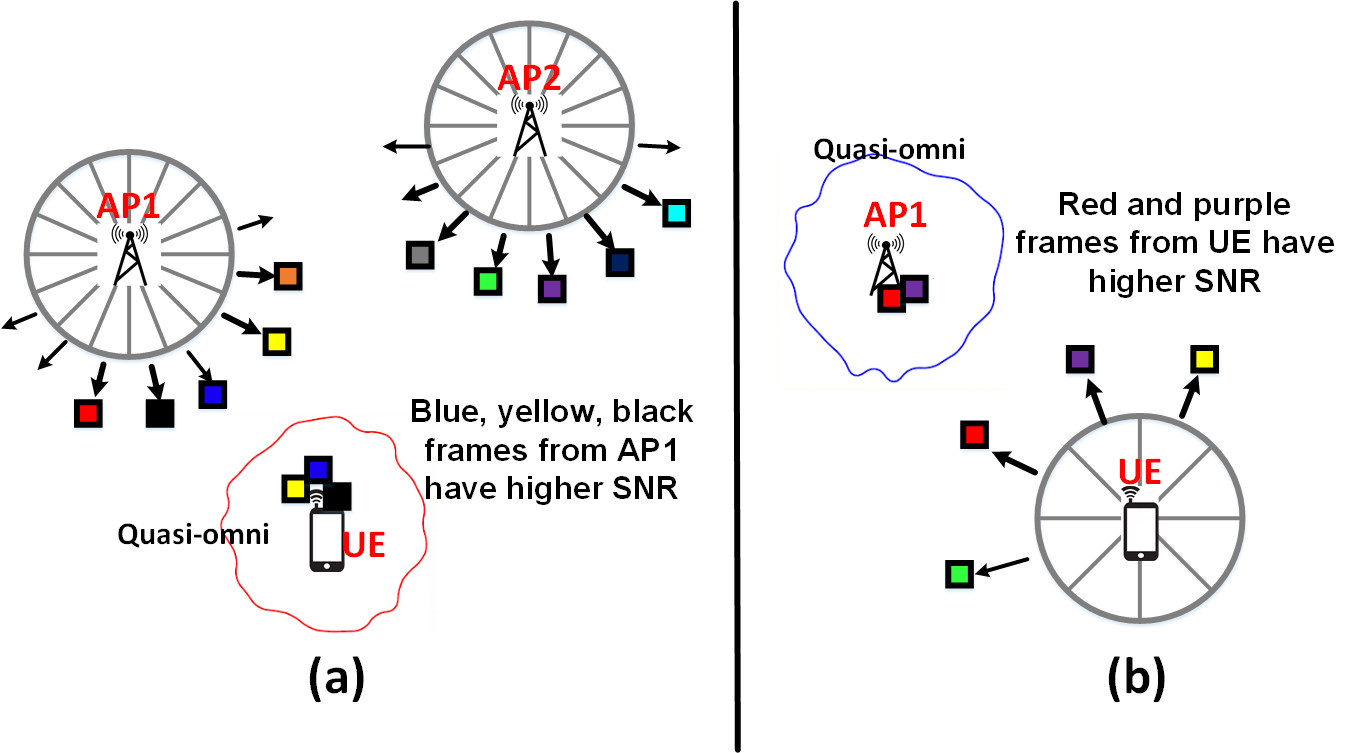
\includegraphics[width=7.5cm,height=4cm]{sls}}
	\caption[U-example]{Sector Level Sweep phase}
\end{figure}
\begin{figure}
	\centerline{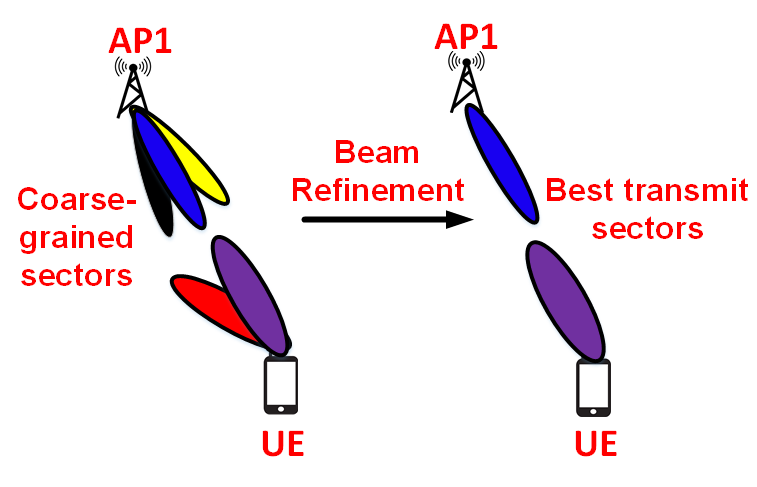
\includegraphics[width=6.5cm,height=4cm]{brp}}
	\caption[U-example]{Beam Refinement phase}
\end{figure}
\begin{figure}
	\centerline{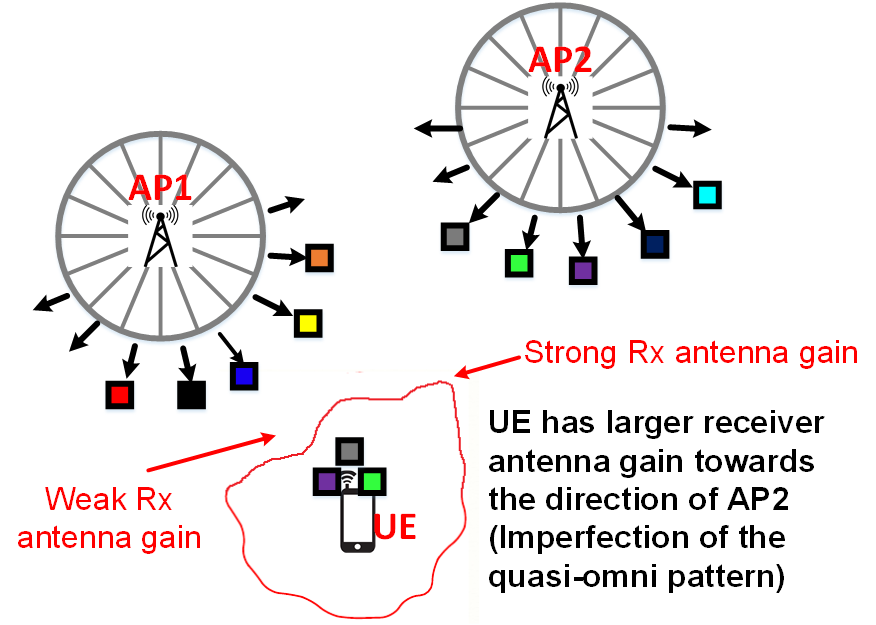
\includegraphics[width=7.5cm,height=5cm]{quasiproblem}}
	\caption[U-example]{Bias caused by quasi-omni-directional antenna pattern}
\end{figure}
\begin{figure}[t!]
	\centerline{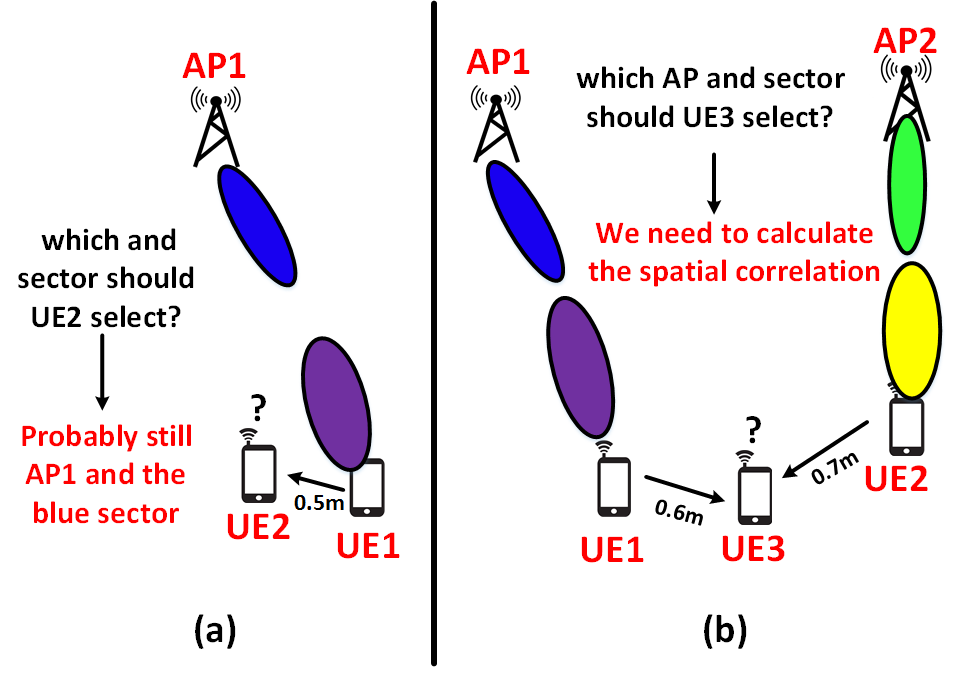
\includegraphics[width=7.5cm,height=5cm]{motivation}}
	\caption[U-example]{Spatial correlation on the AP and sector selection}
\end{figure}
\begin{figure}[t!]
	\centerline{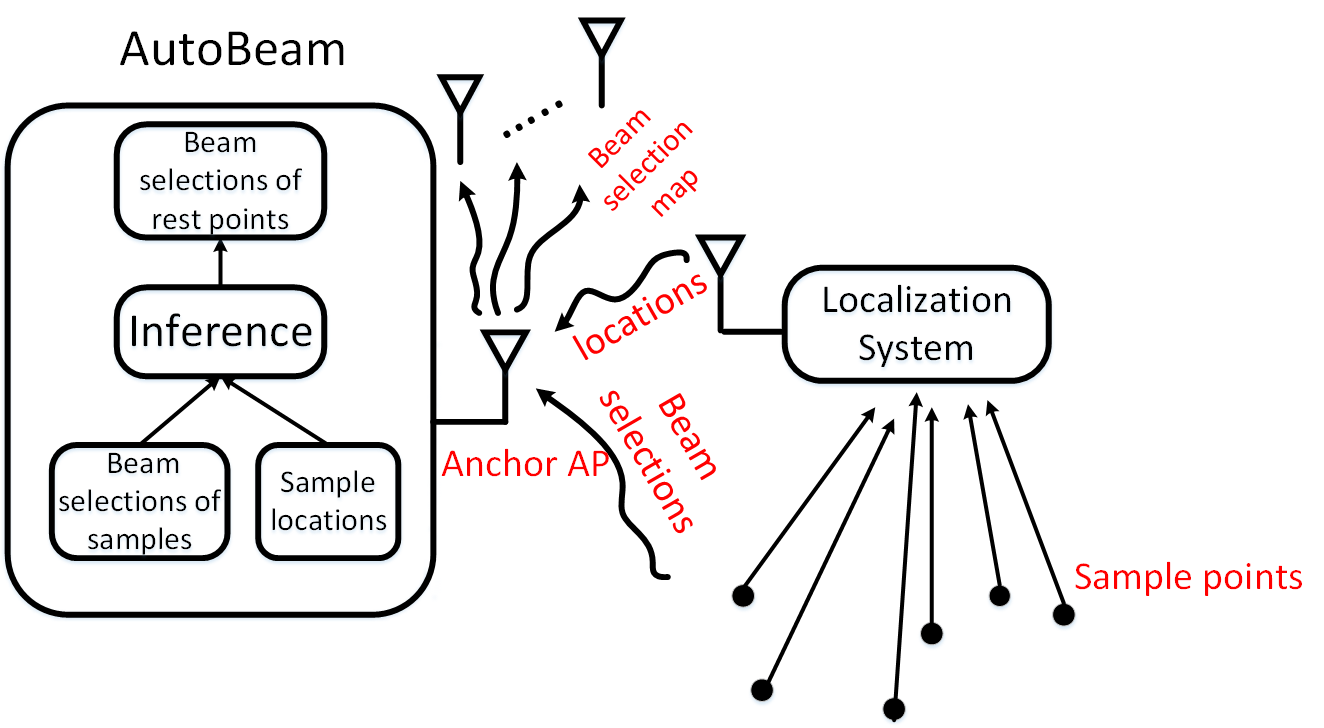
\includegraphics[width=8.5cm,height=5cm]{architecture}}
	\caption[U-example]{Architecture of AutoBeam}
\end{figure}
%\begin{figure}
%\centerline{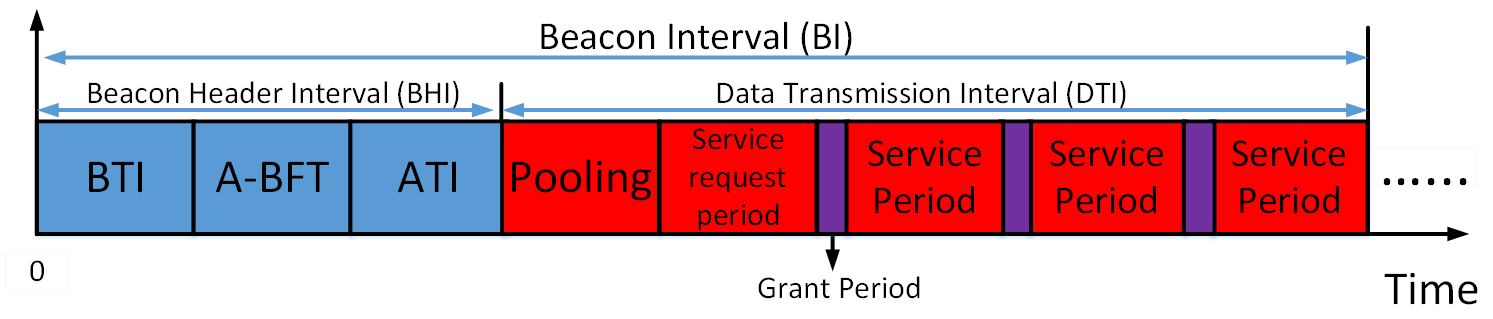
\includegraphics[width=8.5cm,height=2cm]{beaconinterval}}
%\caption[U-example]{IEEE 802.11ad Beacon Interval}
%\end{figure}
\section{Architecture of \emph{AutoBeam}}
The architecture of AutoBeam is shown in Figure 5. We assume that both AP and UE can operate in dual band 5GHz (WiFi) and 60 GHz (mm-wave). For the ease of interpretation, we call the antenna selection, AP transmit sector selection and UE transmit sector selection\emph{beam selection}. In the beginning, several widely distributed samples points are taken at some fixed location in 3D space, and their optimal beam selection is measured by using 802.11ad standard. A localization system returns the rough positions of these sample points. %Typical we assume that the localization error is within 1m for a 10m by 10m by 3m space, which is very reasonable for the current localization system. 
AutoBeam will take the positions as well as the beam selection of these sample points, and returns a list of the beam selections which are ranked in descending order by their probability for the rest of the points in this 3D space. %We further call the mapping between each coordinates in the 3D space and its optimal beam selection \emph{beam selection map}. 
The inference mechanism of AutoBeam can be implemented at any one of the APs, we call this AP the \emph{Anchor AP}. Anchor AP will send the list of beam selections to rest of the APs with WiFi. Assume a UE is making connection with AP with WiFi (Figure 6(a)) and attempts to switch to mm-wave band, it will broadcast a connection request to all the APs with WiFi (Figure 6(b)). Each AP will receive the connection request and the AP and its transmit sector with the highest probability in the list will send test frame to UE, UE will send ACK frame to indicate whether the the frame is received, if UE does not receive the frame, the next best AP and its transmit sector will be used and so forth, until the UE receives test frame from AP, the similar procedure is done for transmission from UE to AP, UE will try its every sector based on the ranking from the list, until the appropriate sector is found (Figure 6(c)). Then AP and UE will proceed to beam refinement phase, and finally communication will be set up (Figure 6(d)). Since a rough estimate for the transmit sectors is returned by AutoBeam, the SLS phase can be skipped.   

In case of mobile UE, a localization system will track the moving devices and return its rough location to all APs through WiFi band. AutoBeam will infer its best beam selection based on the location of UE. And a similar procedure as above is done. 
%The best AP from beam selection map will send the updated optimal sector ID to UE through WiFi. The selected AP and UE will connect by using the updated Tx sectors. 
Given the localization latency of modern localization system is normally within 0.1s[], and whole SLS phase can be skipped, we believe that this tradeoff is reasonable. 
\begin{figure}
	\centerline{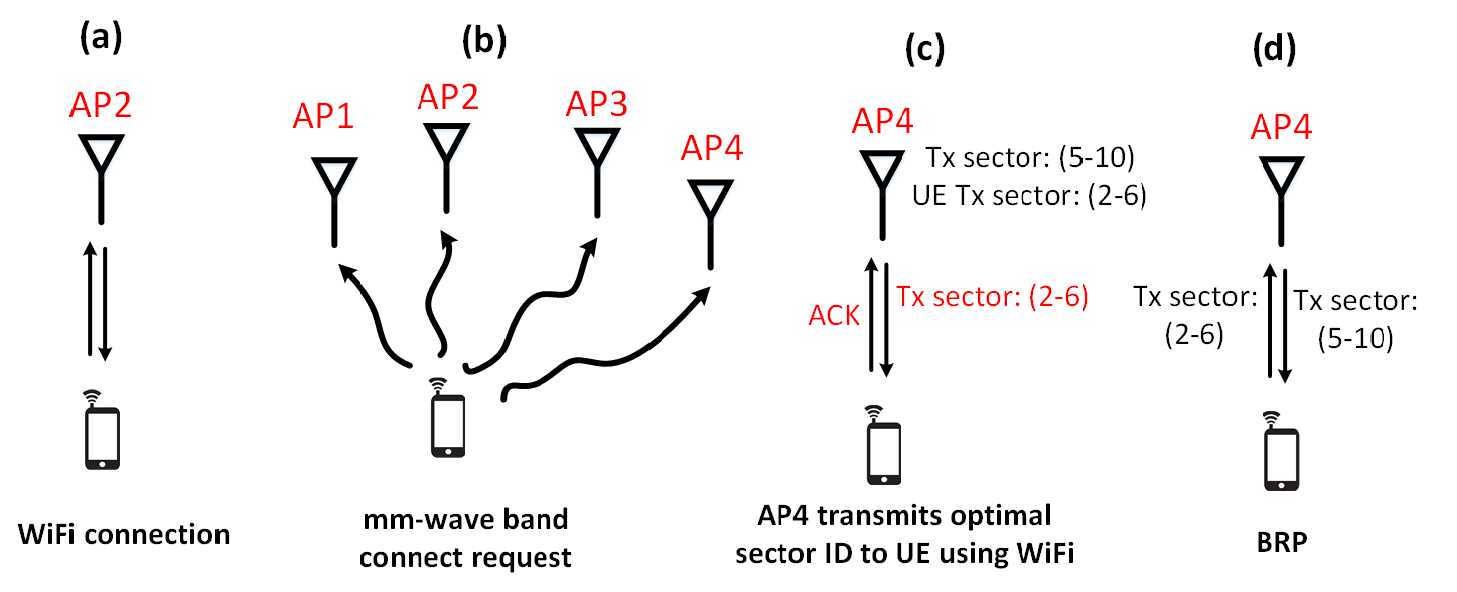
\includegraphics[width=8.5cm,height=4cm]{connection_protocol}}
	\caption[U-example]{Connection Protocol}
\end{figure}

%%%%%%%%%%%%%%%%%%%%%%%%%%%%%%%%%%%%%%%%%%%%%%%%%%%%%%%%%%%%%%%%%%%%%%%%%
%%%%%%%%%%%%%%%%%%%%%%%%%%%%%%%%%%%%%%%%%%%%%%%%%%%%%%%%%%%%%%%%%%%%
\section{CRF Inference Mechanism}
In this section, we will introduce the CRF, and describe how CRF do inference and training. Finally, we will present how CRF will be deployed in AutoBeam.
\subsection{Introduction of CRF}
CRF a type of undirected probabilistic graphical model which is used to encode known relationships between observations and construct consistent interpretations [wikipedia]. To build undirected graphical model for the 3D space, we partitioned 3D space into $a\times b\times c$ small blocks, and $a\times b\times c$ 3D-grid is used to represent the beam selection for each small block (Figure 8). Each node is associated with a random variable which represents the beam selection for this small block. An example is shown in Figure 8. Furthermore, each node and edge of 3D grid are associated with a \emph{node potential} and \emph{edge potential}. In reality, adjacent nodes are tend to have the same beam selection. We capture this tendency using edge potential functions. In addition to this, we have certain “measurements” for the nodes which also influence our belief about their true values. These measurements are represented using node potentials.

Let $x_{v}$ be the beam selection for node $v\in V$, and $x_{V}=\{x_{v\in V}\}$ to represent the beam selection for all the points . By convention, we use $\phi{x_{v}},\psi(x_{v},x_{v'}),$ to denote the node potential of $x_{v}$ and edge potential of $(v,v')\in E$. Given a CRF which is represented by $G(V,E)$, the joint probability $p(x_{V})$ is defined as the product of node potentials and edge potentials:
\begin{equation}
P(x_V)=\frac{1}{Z}\prod_{v\in V} \phi(x_{v})\prod_{(v,v')\in E} \psi(x_{v},x_{v'})
\end{equation} 
Where $Z$ is the normalization constant. 
\subsection{A General Problem}
In this section, we try to solve a general problem: partition the 3D space into $a\times b\times c$ small blocks, and build a $a\times b\times c$ 3D grid, each node in the grid represent the optimal label (either antenna ID or sector ID) for this small block. Given a $a\times b\times c$ 3D grid as described above, and ground truth labels $x_{S}$ of some sample points taken at some fix locations $S$ in the grid, infer the optimal labels for the rest of points in the grid.
Before making the formal definition, we first give a definition on \emph{physical-hops (p-hops)}. Given a point $T$ in the 3D grid, rank the rest of the points in the 3D grid based on its line of sight distance from $T$, the rank of a point $T'$ in this list is called the distance in \emph{physical-hops} between $T'$ and $T$. An example is shown in Figure 7. For the red node in the center, the blue, yellow, purple, green nodes are 1,2,3,4 p-hops away from it. 

Next, we make a formal definition for the node potential and edge potential. We denote $X$ the set of labels, and $x_{v} \in X$ as the optimal label choice of node $v$. The node potential and edge potential are defined as follows:
\begin{equation}
\phi(x_{v})=exp(\sum_{k=0}^{K} w_{k} \sum_{\{s\in S| d(s,v)=k\}} \mathbbm{1}(x_{s}=x_{v}))
\end{equation} 
\begin{equation}
\psi(x_{v},x_{v'})=exp(m_{ij}\mathbbm{1}(x_{v}\neq x_{v'}))
\end{equation} 

Where $w_{k}$ is a measure of correlation on the label selection between a node and the nodes $k$ p-hops away from it, and $K$ is the range of distances in p-hops.  When $k=0$, $w_k$ will be infinity. $S$ is set of sample points taken at some fixed locations in the grid. $d(s,v)$ is the distance in p-hops between node $s$ and $v$. $m_{ij}$ is a parameter which measures degree of penalty for nearby similar nodes that are assigned different labels. By the definition of edge potential, we have $\psi(x_{v},x_{v'}) = exp(m_{ij})$ if $x_{v}\neq x_{v'})$ and $\psi(x_{v},x_{v'}) = 1$ otherwise. By making $m_{ij}$ small, we require the high consistency on label selection between consecutive nodes by making the edge potential$=exp(m_{ij})$ to be small when $x_{v}\neq x_{v'})$, and vice versa. The node potential $\phi(x_{v})$ considers the sample points which are within $K$ p-hops from the node $v$, calculate the weighted sum of number of samples which have the same label as $v$, then take the exponential of it to make sure the node potential is positive. Substitute $(2),(3)$ into $(1)$, we have $p(x_{V}|rm)$, the joint probability of label selection for $x_V$ given 3D space $rm$:
\begin{multline}
P(x_{V}|rm)=\\
\frac{1}{Z}\prod_{v\in V} exp(\smashoperator{\sum_{k=0}^{K}} w_{k} \smashoperator{\sum_{\substack{s\in S\\ d(s,v)=k}}} \mathbbm{1}(x_{s}=x_{v})) \smashoperator{\prod_{(v,v')\in E}}exp(m_{vv'}\mathbbm{1}(x_{v}\neq x_{v'}))
\end{multline} 
%\begin{multline}
%p(x_{V}|r)=
%E_{s}(E_{r}(\frac{1}{Z}\prod_{v\in V} exp(\smashoperator{\sum_{k=0}^{K}} w_{k}  \smashoperator{\sum_{\substack{s\in S\\ %d(s,v)=k}}} \mathbbm{1}(x_{s}=x_{v})) \smashoperator{\prod_{(v,v')\in E}}\\exp(m_{vv'}\mathbbm{1}(x_{v}\neq x_{v'}))))
%\end{multline} 
%Furthermore, we assume that all the samples are taken in rooms $r$ with similar layout, thus $r$ does not affect $w_{k}$ by a lot. We have shown this by simulation in Part ?. Therefore And $p(x_{V})$ equals:
\subsection{CRF Inference} 
In this section, we try to solve the following problem, given the joint probability defined in $(4)$, and parameters  $\theta=\{w_{k},m_{vv'}\} \forall 1\leq k\leq K$ and $(v,v')\in E$, as well as the ground truth labels $x_{S}$ of sample points $S$, infer the optimal labels for the rest of the points in the grid. More specifically, we want to find $x'_{V}$ such that: 
\begin{equation}
x'_{V} = \underset{x_{V}\in X^{|V|}} {argmax}  \quad p(x_{V}|rm)
\end{equation}
Instead of computing the exact distribution $P(x_{V}|rm)$, we will use the mean field approximation to compute $Q(x_{V}|rm) = \prod_{v\in V} Q(x_{v}|rm)$ such that the KL-divergence $D_{KL}(Q||P)$ is minimized, given that $Q(x_{v}|rm)$ to be valid distributions. Therefore we have the following problem: 
\begin{equation}
\underset{Q(x_{v}|rm)}{minimize} \sum_{x_{V}} Q(x_{V}|rm)log(\frac{Q(x_{V}|rm)}{P(x_{V}|rm)})
\end{equation}
\begin{equation}
 s.t.  \sum_{x_{v}} Q(x_{v}|rm)=1 \quad \forall v\in V
\end{equation}
And we have the following iterative updating equations:
\newtheorem{mydef1}{Theorem}
\begin{mydef1}
    $Q(x_{v}|rm), v\in V$ can be calculated by using the following iterative updating equations: 
    \begin{multline}
    Q^{t+1}(x_{V}|rm) =\\
     \frac{exp \Bigg( \smashoperator{\sum_{\substack{v\in V}}}\sum_{k=0}^{K}w_{k} \smashoperator{\sum_{\substack{\{s|d(s,v)=k\}}}} \mathbbm{1}_{x_{s}=x_{v}}+ \smashoperator{\sum_{v'\in N(v)}}Q^{t}(x_{v}|rm)m_{vv'} \mathbbm{1}_{x_{v}\neq x_{v'}}\Bigg)}{\smashoperator{\sum_{x_{v}}} exp \Bigg(\smashoperator{\sum_{\substack{v\in V}}}\sum_{k=0}^{K}w_{k} \smashoperator{\sum_{\substack{\{s|d(s,v)=k\}}}} \mathbbm{1}_{x_{s}=x_{v}}+ \smashoperator{\sum_{v'\in N(v)}}Q^{t}(x_{v}|rm)m_{vv'} \mathbbm{1}_{x_{v}\neq x_{v'}}\Bigg)} 
    \end{multline}
    Where $N(v)$ is the set of neighbors nodes of $v$.
\end{mydef1}
\begin{proof}
	We solve the optimization problem defined by calculating its lagrangian, denote $\widetilde{\phi}(x_{v})
	=\sum\limits_{k=0}^{K}w_{k} \sum\limits_{\substack{s\in S, d(s,v)=k}} \mathbbm{1}_{x_{s}=x_{v}}$ and $\widetilde{\psi}(x_{v},x_{v'})=\mathbbm{1}_{x_{v}\neq x_{v'}}$. We have $P(x_{V}) = \frac{1}{Z} exp(-\sum_{v\in V} \widetilde{\phi}(x_{v})-\sum_{(v,v')\in E} \widetilde{\psi}(x_{v},x_{v'}))$ and $log P(x_{V})=-logZ-\sum_{v\in V} \widetilde{\phi}(x_{v})-\sum_{(v,v')\in E} \widetilde{\psi}(x_{v},x_{v'})$.  And $(6)$ equals:
	 \begin{align*}
	  &\sum_{x_{V}} Q(x_{V}|rm)log(Q(x_{V}|rm))-\sum_{x_{V}} Q(x_{V}|rm)log(P(x_{V}|rm))\\
	  &= \sum_{x_{V}} Q(x_{V}|rm)\sum_{v\in V}log(Q(x_{v}|rm))+ \sum_{x_{V}}Q(x_{V}|rm)(-logZ \\&+ \sum_{v\in V} \widetilde{\phi}(x_{v})+\sum_{(v,v')\in E} \widetilde{\psi}(x_{v},x_{v'}))
     \end{align*}
     \begin{align*} 
     &\text{The Lagrangian } L(x_{V},\lambda_{v}) =  \sum_{x_{V}} Q(x_{V}|rm)\sum_{v\in V}log(Q(x_{v}|rm))\\& +\sum_{x_{V}}Q(x_{V}|rm)(-logZ + \sum_{v\in V} \widetilde{\phi}(x_{v})+\sum_{(v,v')\in E} \widetilde{\psi}(x_{v},x_{v'})) + \\& \lambda_{v} (1-\sum_{x_{v}}Q(x_{v}|rm)) = \sum_{v\in V} \sum_{x_{v}} Q(x_{v}|rm)log(Q(x_{v}|rm)) + \\&\sum_{v\in V}\sum_{x_{v}}Q(x_{v}|rm)\widetilde{\phi}(x_{v})+\sum_{(v,v')\in E}\sum_{x_{v}}\sum_{x_{v'}}Q(x_{v}|rm)Q(x_{v'}|rm)\\&\widetilde{\psi}(x_{v},x_{v'})-logZ.
     \end{align*}
      Take the derivative w.r.t $Q(x_{v}|rm)$, we get $\frac{\partial L(x_{V},\lambda_{v})}{\partial Q(x_{v}|rm)} = -\widetilde{\phi}(x_{v}) - \sum_{v'\in N(v)} Q(x_{v'}|rm) \widetilde{\psi}(x_{v},x_{v'})) +logQ(x_{v}|rm) + 1 -\lambda_{v} = 0$ and $Q(x_{v}|rm)\propto exp(\sum_{v\in V} \widetilde{\phi}(x_{v}) + \sum_{v'\in N(v)} Q(x_{v'}|r)\widetilde{\psi}(x_{v},x_{v'}))$. 
     
     Substitute the definition for $\widetilde{\phi}(x_{v})$ and $\widetilde{\psi}(x_{v},x_{v'})$ to the last equation and normalize the upper equation, we have the update equation defined in $(8)$.
\end{proof}

And the optimal label $x'_{V}$ can be inferred by finding $x'_{v}$ for each $v\in V$ and concatenate together.
%\newtheorem{mydef1}{Theorem}
 \begin{mydef1}
 	Given $Q(x_{V}|rm) = \prod\limits_{v\in V} Q(x_{v}|rm)$ generated by the mean-field approximation defined in $(8)$, we have $x'_{V} = \underset{x_{V}} {argmax}  \quad P(x_{V}|rm) \approx \underset{x_{V}} {argmax}  \quad Q(x_{V}|rm)= \{x_{v}, v\in V\}$, where $x_{v} = \underset{x_{v}} {argmax} \quad Q(x_{v}|rm), \forall v\in V$.
 \end{mydef1}	
 \begin{proof}
 	$x'_{V} = \underset{x_{V}} {argmax} P(x_{V}|rm) \approx \underset{x_{V}} {argmax}  Q(x_{V}|rm) = \underset{x_{V}} {argmax}\prod\limits_{v\in V} Q(x_{v}|rm)$. Therefore $x'_{V} = \{x'_{v}, v\in V\}$, where $x'_{v}$ maximizes $Q(x_{v}|rm)$. 
 \end{proof}
 
 
\subsection{CRF Learning}
Next, we discuss the training for the CRF. Our objective is to find the parameter $\theta=\{w_{k},m_{vv'}\}$,$\forall 1\leq k\leq K$ and $(v,v')\in E$, given the training set $D=\{D^{1},D^{2},...,D^{R}\}$. $D^{r}$ is a $a\times b\times c$ matrix which contains the optimal labels for the 3D grid measured from 3D space $rm_{r}$. We assume that all the 3D-space $1\leq r\leq R$ have similar dimension and layout (e.g. different one bedroom condos) To generate these optimal labels, we partition the 3D space into $a\times b\times c$ small blocks and get the optimal label for each small block. We are not interested in $w_{0}$ since $w_0$ equals infinity theoretically, instead we set $w_{0}$ to a very large number. We have the following derivation for the posterior distribution $p(\theta|D)$.
\begin{align}
&\prod_{r=1}^{R} P(D^{r}|rm_{r},\theta) P(\theta)= \prod_{r=1}^{R} P(D^{r}|rm_{1},...,rm_{R},\theta)P(\theta) \\
 &=P(D|rm_{1},...,rm_{R},\theta) P(\theta)\\
&= P(D|rm,\theta)p(\theta) \propto P(\theta|rm,D)
\end{align}
$(9)$ follows from the fact that $rm_{i}$ is independent with $D^{j}$ for $i\neq j$. The second equality follows from the fact that $\{D^{i}\},(1\leq i\leq R) $ is conditionally independent given $rm_{1},...,rm_{R}$.The third equality follows from the assumption that all the 3D spaces have similar layout and dimension, hence can be represented by a single variable $rm$. The last equality follows from the Bayesian rule. Without loss of generality, We further assume that the prior of $\theta=\{w_k, m_{vv'}\}$ follow a Gaussian distribution with mean $\mu_{w_{k}}$, $\mu_{m_{vv'}}$ and standard deviation $\sigma_{w_{k}}$, $\sigma_{m_{vv'}}$ respectively. Therefore we have the following definition for the prior distribution. 
\begin{align*}
    P(\theta) &= \prod_{k=1}^{K} P(w_{k}) \prod_{(v,v')\in E} P(m_{vv'})\\ &= \prod_{k=1}^{K} \mathcal{N}(w_{k};\mu_{w_{k}},\sigma_{w_{k}})\prod_{(v,v')\in E}\mathcal{N}({m}_{vv'};\mu_{m_{vv'}},\sigma_{m_{vv'}})\numberthis 
\end{align*}
Where $\mathcal{N}(x;\mu,\sigma)$ represents the Gaussian pdf with variable $x$, mean $\mu$ and standard deviation $\sigma$. Then we substitute $(4)$ and $(12)$ to $(11)$, we have 
%\begin{equation}
\begin{align*}
    &\frac{1}{R}log P(\theta|rm,D) = \frac{1}{R}\sum_{r=1}^{R}log P(D^{r}|rm_{r},\theta) + \frac{1}{R}log  P(\theta)+ C\\&= -\frac{1}{R}\sum_{r=1}^{R}logZ_{rm}^{r}(\theta) + \frac{1}{R}\sum_{r=1}^{R}\bigg(\sum_{v\in V}\sum_{k=0}^{K}w_{k}\smashoperator{\sum_{\{s|d(s,v)=k\}}} \mathbbm{1}_{x^{r}_{s}=x^{r}_{v}} + \\& \smashoperator{\sum_{(v,v')\in E}} m_{vv'} \mathbbm{1}_{x^{r}_{v}\neq x^{r}_{v'}} \bigg)+ \frac{1}{R} \sum_{k=0}^{K} -\frac{(w_{k}-\mu_{w_{k}})^{2}}{2\sigma_{w_{k}}^{2}} + \\& \frac{1}{R} \smashoperator{\sum_{(v,v')\in E}} -\frac{(m_{vv'}-\mu_{m_{vv'}})^{2}}{2\sigma_{m_{vv'}}} + C \numberthis 
\end{align*}
Where $Z_{rm}^{r}(\theta)$ is the normalization constant for $p(D^{r}|rm_{r},\theta)$, $x^{r}_{v}$,$x^{r}_{s}$ is label of $v$ and $s$ in $D^{r}$ and $C$ is constant. Given the expression for the posterior distribution, we want to find $\theta'$ which maximize $(13)$. We have the following theorem:
\begin{mydef1}
	We have the following equations for gradient: \\
 $\frac{\partial \frac{1}{R}log P(\theta|rm,D)}{\partial w_{k}}= E_{D}(\sum_{v\in V} \sum_{\{s|d(s,v)=k\}} \mathbbm{1}_{x_{s}=x_{v}})-\frac{1}{R} \sum_{r=1}^{R}E_{P(x_{V}|rm_{r};\theta)}(\sum_{\{s|d(s,v)=k\}} \mathbbm{1}_{x_{s}=x_{v}}) + \frac{\mu_{w_{k}}-{w}_{k}}{R\sigma_{w_{k}}^{2}}$ and  $\frac{\partial \frac{1}{R}log P(\theta|rm,D)}{\partial m_{vv'}}= E_{D}(\mathbbm{1}_{x_{v}\neq x_{v'}}) -\frac{1}{R} E_{P(x_{V}|rm_{r};\theta)} (\mathbbm{1}_{x_{v}\neq x_{v'}})+\frac{\mu_{m_{vv'}}-m_{vv'}}{R\sigma_{m_{vv'}}^{2}}$, where $E_{D}(.)$ is the empirical expectation over the training data $D$ and $E_{P(x_{V}|rm_{r};\theta)}(.)$ is the expectation over $P(x_{V}|rm_{r},\theta)$. 
\end{mydef1}
 \begin{proof}
     Remove all the items which do not contain $w_{k}$ out of $(13)$, $(13)$ can be written as 
     $\underbrace{-\frac{1}{R}\sum_{r=1}^{R}logZ_{rm}^{r}(\theta)}_{Part A}$ +  $\underbrace{\frac{1}{R}\sum_{r=1}^{R}\sum_{v\in V}\sum_{k=0}^{K}w_{k}\smashoperator{\sum_{\{s|d(s,v)=k\}}} \mathbbm{1}_{x^{r}_{s}=x^{r}_{v}}}_{Part B} + \underbrace{\frac{1}{R} \sum_{k=0}^{K} -\frac{(w_{k}-\mu_{w_{k}})^{2}}{2\sigma_{w_{k}}^{2}}}_{Part C} + C$, we have $\frac{\partial Part A}{\partial w_{k}} = -\frac{1}{R}\sum_{r=1}^{R} \frac{\partial logZ_{rm}^{r}(\theta)}{\partial w_{k}}$, since $Z_{rm}^{r}(\theta)$ is the normalization constant for $P(D^{r}|rm_{r},\theta)$, we have 
     
     $Z_{rm}^{r}(\theta) = \smashoperator{\sum_{x_{V}}} exp\bigg(\smashoperator{\sum_{v\in V}}\smashoperator{\sum_{k=0}^{K}} w_{k} \smashoperator{\sum_{\substack{\{s|d(s,v)=k\}}}} \mathbbm{1}_{x_{s}=x_{v}})+\smashoperator{\sum_{(v,v')\in E}} m_{vv'}\mathbbm{1}_{x_{v}\neq x_{v'}}\bigg)$.Therefore we have the following derivation:
     \begin{align*}
     &\frac{\partial log(Z_{rm}^{r}(\theta))}{\partial w_{k}} =\frac{1}{Z_{rm}^{r}(\theta)}\frac{\partial Z_{rm}^{r}(\theta)}{\partial w_{k}} = \sum\limits_{x_{V}} \sum\limits_{v\in V}\sum\limits_{\{s|d(s,v)=k\}} \\&\mathbbm{1}_{x_{s}=x_{v}}  \frac{1}{Z_{rm}^{r}(\theta)}exp(\sum\limits_{v\in V}\sum\limits_{k=0}^{K} w_{k} \sum\limits_{\substack{\{s|d(s,v)=k\}}} \mathbbm{1}_{x_{s}=x_{v}}+\sum_{(v,v')\in E}\\& m_{vv'}\mathbbm{1}_{x_{v}\neq x_{v'}}) = E_{P(x_{V}|rm_{r};\theta)}\bigg(\sum_{\{s|d(s,v)=k\}} \mathbbm{1}_{x_{s}=x_{v}}\bigg).
     \end{align*}
      Hence we got $\frac{\partial Part A}{\partial w_{k}} = -\frac{1}{R}\sum_{r=1}^{R} E_{P(x_{V}|rm_{r};\theta)}\bigg(\sum_{\{s|d(s,v)=k\}} \mathbbm{1}_{x_{s}=x_{v}}\bigg)$. By taking derivative w.r.t Part B, we get $\frac{\partial Part B}{\partial w_{k}} = \frac{1}{R}\sum_{r=1}^{R}\sum_{v\in V}\sum_{\{s|d(s,v)=k\}} \mathbbm{1}_{x^{r}_{s}=x^{r}_{v}} = E_{D}\bigg(\smashoperator{\sum_{v\in V}} \sum_{\{s|d(s,v)=k\}} \mathbbm{1}_{x_{s}=x_{v}}\bigg)$. Finally we have $\frac{\partial Part C}{\partial w_{k}} = \frac{\mu_{w_{k}}-{w}_{k}}{R\sigma_{w_{k}}^{2}}$, summing them together gives first part of theorem 3. To prove second part, we rewrite $(12)$ as $\underbrace{-\frac{1}{R}\sum_{r=1}^{R}logZ_{rm}^{r}(\theta)}_{Part A}$ +  $\underbrace{\frac{1}{R}\sum_{r=1}^{R} \smashoperator{\sum_{(v,v')\in E}} m_{vv'} \mathbbm{1}_{x^{r}_{v}\neq x^{r}_{v'}}}_{Part B} + \underbrace{\frac{1}{R} \sum_{k=0}^{K} -\frac{(m_{vv'}-\mu_{m_{vv'}})^{2}}{2\sigma_{m_{vv'}}^{2}}}_{Part C} + C$, by carrying out the similar step as above, we get $\frac{\partial Part A}{\partial m_{vv'}} = -\frac{1}{R} E_{P(x_{V}|rm_{r};\theta)} (\mathbbm{1}_{x_{v}\neq x_{v'}}), \frac{\partial Part B}{\partial m_{vv'}} = E_{D}(\mathbbm{1}_{x_{v}\neq x_{v'}})$ and $\frac{\partial Part C}{\partial m_{vv'}} =\frac{\mu_{m_{vv'}}-m_{vv'}}{R\sigma_{m_{vv'}}^{2}}$, summing them together gives the second part of theorem 3.
 \end{proof}
After finding the gradient of the posterior distribution w.r.t $\theta$, we can find the optimal $\theta$ by using gradient ascent method, which is described in Algorithm 1. 

\begin{algorithm}[H]
	Input: $\theta^{(0)}=\{w_{k}^{(0)},m_{vv'}^{(0)}\},\forall 1\leq k\leq K, (v,v')\in E$, step size $\eta$, stopping criterion $\Delta$, maximum number of iteration $I_{max}$, training data $D$ \\
	Output: $\theta^{*}=\{w_{k}^{*},m_{vv'}^{*}\},\forall 1\leq k\leq K, (v,v')\in E$, which maximizes $(13)$ \\
	\For{i=1,...,$I_{max}$}{ 
		Compute\\ $\frac{\partial \frac{1}{R}log P(\theta|rm,D)}{\partial \theta} = \{\frac{\partial \frac{1}{R}log P(\theta|rm,D)}{\partial w_{k}},\frac{\partial \frac{1}{R}log P(\theta|rm,D)}{\partial m_{vv'}}\}$ with equations of gradients in Theorem 3.\\
		Compute $\theta^{(i)}=\theta^{(i-1)}+ \eta\frac{\partial \frac{1}{R}log P(\theta|rm,D)}{\partial \theta}$\\
		\If{$||\theta^{(i)}-\theta^{(i-1)}||\leq \Delta$}{
			$\theta^{*} = \theta^{i}$ \\
			Break;
		}

}
\caption{Gradient Ascent Algorithm}
\end{algorithm}
Furthermore, theorem 4 states that the parameter $\theta^{*}$ found by Algorithm 1 is the global optimum.  
\begin{mydef1}
	The $\theta^{*}$ returned by Algorithm 1 is the global optimum for the optimization problem $\underset{\theta}{argmax} P(\theta|rm, D)$
\end{mydef1}
\begin{proof}
	We prove that $P(\theta|D,rm)$ is a concave function, therefore the global maximum can be found by using gradient ascent method defined in Algorithm 1. To prove its concavity, first we define random variable $u_{r}^{k}=\sum_{v\in V}\sum_{\substack{\{s|d(s,v)=k\}}}\mathbbm{1}_{x^{r}_{s}=x^{r}_{v}}$, and define $h_{r} = \smashoperator{\sum_{v\in V}}\smashoperator{\sum_{k=0}^{K}} w_{k} \smashoperator{\sum_{\substack{\{s|d(s,v)=k\}}}} \mathbbm{1}_{x^{r}_{s}=x_{v}}+\smashoperator{\sum_{(v,v')\in E}} m_{vv'}\mathbbm{1}_{x_{v}\neq x_{v'}}$, and we use the same definition for Part A, Part B, Part C as the proof for Theorem 3. We have $\frac{\partial^{2} part C}{\partial w_{k} \partial w_{k'}} = -\frac{1}{R\sigma_{w_{k}}^{2}}$ if $k'=k$ and $0$ otherwise, $\frac{\partial^{2} part B}{\partial w_{k} \partial w_{k'}} = 0$, $\frac{\partial^{2} part A}{\partial w_{k} \partial w_{k'}} = -\frac{1}{R}\sum_{r=1}^{R}\sum_{x_{V}}\frac{u_{r}^{k}u_{r}^{k'}exp(h_{r})Z^{r}_{rm}-exp(h_{r})\sum_{x_{V}u_{r}^{k'}exp(h_{r})}}{Z^{r^2}_{rm}} = -\frac{1}{R}\sum_{r=1}^{R}\sum_{x_{V}} u_{r}^{k}u_{r}^{k'} \frac{exp(h_{r})}{Z^{r}_{rm}} -  u_{r}^{k}\frac{exp(h_{r})}{Z^{r}_{rm}} \sum_{x_{V}} u_{r}^{k'}\frac{exp(h_{r})}{Z^{r}_{rm}} = -\frac{1}{R}\sum_{r=1}^{R} E_{p(x_{V}|rm_{r})} (u_{r}^{k} u_{r}^{k'})-E_{p(x_{V}|rm_{r})}(u_{r}^{k}) E_{p(x_{V}|rm_{r})}(u_{r}^{k'}) = -\frac{1}{R}\sum_{r=1}^{R} Cov(u_{r}^{k},u_{r}^{k'})$. We also have $\frac{\partial^{2} part C}{\partial w_{k}\partial m_{vv'}} = \frac{\partial^{2} part B}{\partial w_{k}\partial m_{vv'}} = 0$, and $\frac{\partial^{2} part A}{\partial w_{k}\partial m_{vv'}} = -\frac{1}{R}\sum_{r=1}^{R}Cov(u_{r}^{k},\mathbbm{1}_{x_{v}\neq x_{v'})}$. Similarly, we have $\frac{\partial^{2} part C}{\partial m_{vv'} \partial m_{zz'}} =  -\frac{1}{R\sigma_{m_{vv'}}^{2}}$ if $v=z,v'=z'$ and $0$ otherwise. $\frac{\partial^{2} part B}{\partial m_{vv'} \partial m_{zz'}} = 0$, $\frac{\partial^{2} part A}{\partial m_{vv'} \partial m_{zz'}} = -\frac{1}{R}\sum_{r=1}^{R}Cov(\mathbbm{1}_{x_{v}\neq x_{v'}},\mathbbm{1}_{x_{z}\neq x_{z'}})$, and $\frac{\partial^{2} part C}{\partial m_{vv'} \partial w_{k}} = \frac{\partial^{2} part B}{\partial m_{vv'} \partial w_{k}} = 0$, and $\frac{\partial^{2} part A}{\partial m_{vv'} \partial w_{k}} = -\frac{1}{R}\sum_{r=1}^{R}Cov(\mathbbm{1}_{x_{v}\neq x_{v'}}, u_{r}^{k})$. Hence we have $\frac{\partial^{2} P(\theta|D,rm)}{\partial^{2} \theta} = -\frac{1}{R}\sum_{r=1}^{R} K(\vec{u_{r}},\vec{\mathbbm{1}}_{x_{v}\neq x_{v'}}) + \Phi$, where $\vec{u_{r}} = \{u^{1}_{r},...,u^{K}_{r}\}$ and $\vec{\mathbbm{1}}_{x_{v}\neq x_{v'}} = \{\mathbbm{1}_{x_{v}\neq x_{v'}}\}$, $\forall (v,v')\in E$. $K(\vec{u_{r}},\vec{\mathbbm{1}}_{x_{v}\neq x_{v'}})$ is the covariance matrix between $\vec{u_{r}}$ and $\vec{\mathbbm{1}}_{x_{v}\neq x_{v'}}$. And $\Phi$ is the diagonal matrix $diag(-\frac{1}{R\sigma_{w_{1}}^{2}},...,-\frac{1}{R\sigma_{w_{K}}^{2}},\{-\frac{1}{R\sigma_{m_{vv'}}^{2}}\})$ which has negative constants on the diagonal. Therefore $\Phi$ is a negative semidefinite matrix. Moreover, $-\frac{1}{R}\sum_{r=1}^{R} K(\vec{u_{r}},\vec{\mathbbm{1}}_{x_{v}\neq x_{v'}})$ is a sum of negative covariance matrix, therefore it is also a negative semidefinite matrix. Therefore $\frac{\partial^{2} P(\theta|D,rm)}{\partial^{2} \theta}$ is a negative semidefinite matrix and $P(\theta|D,rm)$ is a concave function in $\theta$.
\end{proof}
\subsection{Prior calculation for $\mu_{w_{k}}$ and $\mu_{m_{vv'}}$ }
In the previous sections, we assume that $P(w_{k})\sim \mathcal{N}(x;\mu_{w_{k}},\sigma_{w_{k}})$ and  $P(m_{vv'})\sim \mathcal{N}(x;\mu_{m_{vv'}},\sigma_{m_{vv'}})$. However, we have not talk about the values for the hyperparameters $\mu_{w_{k}},\mu_{m_{vv'}}$. In this section, we will present a method to calculate them from intuition. 
Consider a node $T$ in a 3D grid which models a indoor environment, and denote $M_{i},1\leq i\leq K$  the set of nodes which are i p-hops away from this node. An 2D version of this example is shown in Figure ?. The node is shown in red and the $M_{1},M_{2},...,M_{4}$ are shown in blue, yellow, purple, green and black respectively. We assume the physical distances between any two consecutive nodes in the grid are the same, which equals $d$, and there is a Tx antenna with omni-directional antenna pattern placed at each node in $M_{i}$. We further assume that each Tx antenna is labeled the same color as the node, so each $M_{i}$ has its specific set of Tx antennas, denoted by $Tx_{i}^{M}$. Assume all the Tx antennas have the same transmit antenna gain, each Tx antenna broadcasts frames with the same transmitting power at mm-wave frequency band. Assume that a Rx antenna with omni-directional antenna pattern is placed at $T$. From [28 GHz and 73 GHz Millimeter-Wave Indoor Propagation Measurements and Path Loss Models], we have the following close-in free space reference path loss model for indoor LOS and NLOS scenario.
\begin{equation}
    PL(d)[dB] = PL_{FS}(d_{0})[dB]+10\bar{n}log_{10}\frac{d}{d_{0}}+X_{\delta}
\end{equation}
Where $PL_{FS}(d_{0})$ is the free space path loss at $d_{0}$, $\bar{n}$ is the \emph{omni-directional path loss exponential}. $X_{delta}$ is the \emph{shadow factor}, which is a normal random variable with 0 mean and standard deviation $\delta$. The pass loss model is obtained by considering the measured power delay profiles (PDP) for each Tx antenna and Rx antenna location combination at every unique pointing angles, then sum over all the PDPs to generate the directional received power as a function of pointing angle, then subtract the Tx antenna gain and Rx antenna gain from the directional received power, finally sum the directional receiver power over every Tx-Rx pointing angle to generate the omni-directional path loss model.
\begin{figure}
	\centerline{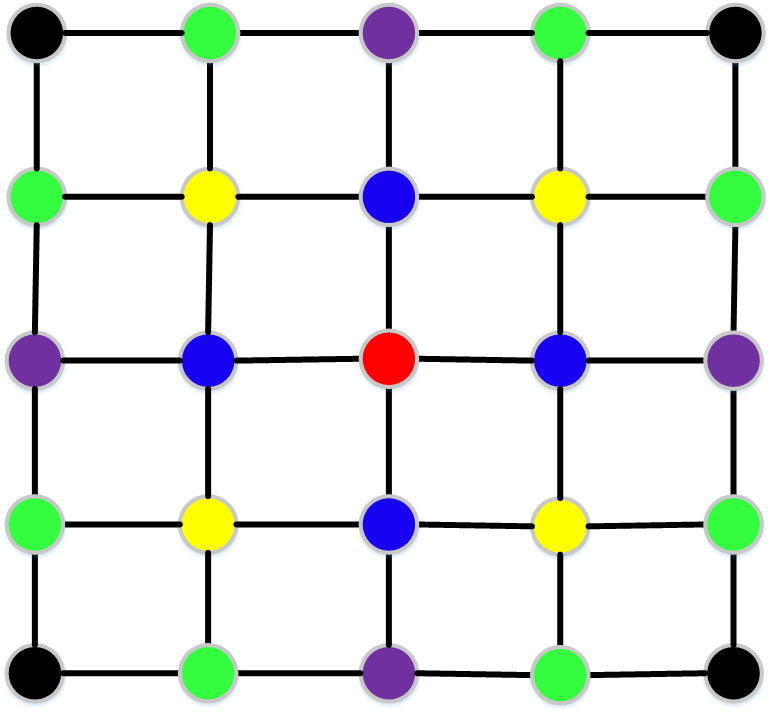
\includegraphics[width=5cm,height=5cm]{grid}}
	\caption[U-example]{An 2D example}
\end{figure}
From [], the path loss exponential $\bar{n}$ and standard deviation $\delta$ for LOS scenario is 1.1, 1.7 at 28GHz and 1.3,1.9 at 73GHz. For NLOS, the path loss exponential $\bar{n}$ and standard deviation $\delta$ is 2.7, 9.6 at 28GHz and 3.2,11.3 at 73GHz. We take the average over the 28GHz and 73Ghz, we have $\bar{n} = 1.2, \delta=1.8$ for LOS and  $\bar{n} = 2.95, \delta=10.45$ for NLOS.

The work done in [] indicates that the probability $P_{blk}$ that the line of sight path between $T$ and every other node is blocked proportional to the physical distance between $T$ and the node. That is, we have:
\begin{equation}
    P_{blk} = P_{e}L 
\end{equation}
Where $P_{e}$ is the blocking probability per unit distance in meter. $L$ is the distance between $T$ and the node. By "line of sight path between $T$ and every other node is blocked", we mean there is a obstruction between them. Furthermore, we assume that line of sight path is blocked happens independently. Since the Tx antenna gain are the same for all the Tx antennas and Rx antenna is omni-directional, the received power at between any other node and $T$ is purely decided by the path loss between them.

From $(8)$, we have 
\begin{equation}
Q^{t+1}(x_{V}|rm) \propto\\
exp \Bigg( \smashoperator{\sum_{\substack{v\in V}}}\sum_{k=0}^{K}w_{k} \smashoperator{\sum_{\substack{\{s|d(s,v)=k\}}}} \mathbbm{1}(x_{s}=x_{v})+ \smashoperator{\sum_{v'\in N(v)}}Q^{t}(x_{v}|rm)m_{vv'} \mathbbm{1}(x_{v}\neq x_{v'})\Bigg)
\end{equation}
Since $Q^{t+1}(x_{V}|rm) = \prod_{v\in V} Q^{t+1}(x_{v}|rm)$. Therefore we have:
\begin{equation}
Q^{t+1}(x_{v}|rm) \propto\\
exp \Bigg( \sum_{k=0}^{K}w_{k} \smashoperator{\sum_{\substack{\{s|d(s,v)=k\}}}} \mathbbm{1}(x_{s}=x_{v})+ \smashoperator{\sum_{v'\in N(v)}}Q^{t}(x_{v}|rm)m_{vv'} \mathbbm{1}(x_{v}\neq x_{v'})\Bigg)
\end{equation}
Ignore the edge potential, we have:
\begin{equation}
Q^{t+1}(x_{v}|rm) \propto\\
exp \Bigg( \sum_{k=0}^{K}w_{k} \smashoperator{\sum_{\substack{\{s|d(s,v)=k\}}}} \mathbbm{1}(x_{s}=x_{v})\Bigg)
\end{equation}
Now consider the scenario described in the beginning of this subsection, there is a Tx antennas at every other node with its unique label $Tx_{i}^{M}$, and each Tx antenna broadcast frames with a omni-directional pattern, the transmitting power are the same and all the Tx antenna gain are the same. Assume that the probability that each line-of-sight path between $T$ and another node is blocked follows $(14)$, and a Rx antenna is located at $T$ and hear with a omni-directional pattern. $T$ will choose the Tx antenna set $Tx_{i}^{M}$ which has the highest average received power to connect. We want to calculate the probability that $T$ chooses $Tx_{i}^{M}$ to connect.  We have:
\begin{equation}
    Q^{t+1}(x_{T}=Tx_{k}^{M}|rm) \propto exp\Bigg( \sum_{k=0}^{K}w_{k} \smashoperator{\sum_{\substack{\{s|d(s,T)=k\}}}} \mathbbm{1}(x_{s}=Tx_{k}^{M})\Bigg)
\end{equation}
\begin{multline}
Q^{t+1}(x_{T}=Tx_{k}^{M}|rm) \propto exp(w_{k}\smashoperator{\sum_{\substack{\{s|d(s,T)=k\}}}}\mathbbm{1}(x_{s}=Tx_{k}^{M})) \\= exp(w_{k}|M_{k}|)
\end{multline}
\begin{equation}
w_{k} = \frac{1}{|M_{k}|} log(Q^{t+1}(x_{T}=Tx_{k}^{M}|rm)) + C
\end{equation}
$(19)$ comes from the fact that all the nodes which has its label $Tx_{k}^{M}$ are k p-hops away and there are $|M_{k}|$ such nodes.

Then we are left with calculating $Q(x_{T}=Tx_{k}^{M}|rm)$, the probability of $x_{T}$ making connection with $Tx_{k}^{M}$. We have the following theorem:
\begin{mydef1}
	Assume all the antennas in $Tx_{k}^{M}$ have the same value for LOS/NLOS shadowing factors. The excepted average received power $E[P_{r}^{k}]$ from $Tx_{k}^{M}$ (in dB) is $log(P_{t}G_{t}G_{r})-PL_{FS}(d_{0})-(17.5P_{e}\tau_{k}d+12)log_{10}(\tau_{k}d)-(X^{NLOS}_{\delta}-X^{LOS}_{\delta})P_{e}\tau_{k}d-X^{LOS}_{\delta}$, where $tau_{k}d$ is the physical distance between nodes in $M_{k}$ and $T$, $X^{NLOS}_{delta}$ is the shadow factor for NLOS and $X^{LOS}_{delta}$ is the shadow factor for LOS, and the expectation is taken over number of blocked line of sight paths .
\end{mydef1}
\begin{proof}
	Let $\rho$ denote the number of blocked paths, since the line of sight path is blocked happens independently, $\rho$ is a binomial random variable with probability $P_{e}\tau_{k}d$. We have the average received power $P_{r}^{k}$, given $\rho$ is $\frac{1}{|w_{k}|}(|w_{k}|log(P_{t}G_{t}G_{r})-\rho(PL_{FS}(d_{0})+29.5log_{10}\tau_{k}d + X^{NLOS}_{delta})-(|w_{k}|-\rho(PL_{FS}(d_{0})+12log_{10}\tau_{k}d + X^{LOS}_{delta}))$, and $P_{r}^{k}$ is a linear function of $\rho$. Hence the expected value of $P_{r}^{k}$ over $\rho$ can be found by substitute $E(\rho) = |w_{k}|P_{e}\tau_{k}d$ to the last equation. After derivation, we have $E[P_{r}^{k}]=log(P_{t}G_{t}G_{r})-PL_{FS}(d_{0})-(17.5P_{e}\tau_{k}d+12)log_{10}(\tau_{k}d)-(X^{NLOS}_{\delta}-X^{LOS}_{\delta})P_{e}\tau_{k}d-X^{LOS}_{\delta}$.
\end{proof}
Given the result of theorem 5, we can calculate the probability $Q(x_{T}=Tx_{k}^{M}|rm)$, the result is stated in theorem 6:
\begin{mydef1}
	Let $X^{LOS}_{\delta_{k}},X^{NLOS}_{\delta_{k}}$ denote the shadow factor for NLOS and LOS of $Tx_{k}^{M}$. Then we have $Q(x_{T}=Tx_{k}^{M}|rm) = \prod_{k'=1,k'\neq k}^{K} \mathcal(Q)(\frac{12log_{10}(\frac{\tau_{k}}{\tau_{k'}})}{1.8\sqrt{2}})$
\end{mydef1}
\begin{proof}
	First, we calculate $P(E[P_{r}^{k}]>E[P_{r}^{k'}])$, the probability of expected average received power from $Tx_{k}^{M}$ is greater that from $Tx_{k'}^{M}$. By using the result of theorem 5. We have:
	\begin{multline}
	P(E[P_{r}^{k}]>E[P_{r}^{k'}]) =\\ P(log(P_{t}G_{t}G_{r})-PL_{FS}(d_{0})-(17.5P_{e}\tau_{k}d+12)log_{10}(\tau_{k}d)-(X^{NLOS}_{\delta_{k}}-X^{LOS}_{\delta_{k}})P_{e}\tau_{k}d-X^{LOS}_{\delta_{k}}>\\log(P_{t}G_{t}G_{r})-PL_{FS}(d_{0})-(17.5P_{e}\tau_{k'}d+12)log_{10}(\tau_{k'}d)-(X^{NLOS}_{\delta_{k'}}-X^{LOS}_{\delta_{k'}})P_{e}\tau_{k'}d-X^{LOS}_{\delta_{k'}})
	\end{multline}
	After cancellation, we have the upper probability equal to:
	\begin{equation}
	P(X^{LOS}_{\delta_{k'}}-X^{LOS}_{\delta_{k}}+P_{e}d(\tau_{k'}X^{NLOS}_{\delta_{k'}}- \tau_{k'}X^{LOS}_{\delta_{k'}}-\tau_{k}X^{NLOS}_{\delta_{k}}+ \tau_{k}X^{LOS}_{\delta_{k}})>17.5P_{e}d(\tau_{k}log_{10}(\tau_{k}d)-\tau_{k'}log_{10}(\tau_{k'}d))+12log_{10}(\tau_{k}d)-12log_{10}(\tau_{k'}d))
	\end{equation}
	To make the prediction on every location in the 3D space, we want to partition the 3D space into infinite small blocks. which means the physical distance $d$ between two nodes in the grid is zero ideally. Moreover, from [], $P_e$ is also a very small $(\approx 0.0078)$, therefore we have $P_{e}d \approx 0$, and we get:
	\begin{equation}
	    P(E[P_{r}^{k}]>E[P_{r}^{k'}]) = P(X^{LOS}_{\delta_{k'}}-X^{LOS}_{\delta_{k}}>12log_{10}(\tau_{k}d)-12log_{10}(\tau_{k'}d))=
	    P(X^{LOS}_{\delta_{k'}}-X^{LOS}_{\delta_{k}}>12log_{10}(\frac{\tau_{k}}{\tau_{k'}})
	\end{equation}
	Since $X^{LOS}_{\delta_{k'}},X^{LOS}_{\delta_{k}}\sim \mathcal(N)(0,1.8)$, we have $X^{LOS}_{\delta_{k'}}-X^{LOS}_{\delta_{k}}\sim \mathcal(N)(0,1.8\sqrt{2})$, hence $P(E[P_{r}^{k}]>E[P_{r}^{k'}]) = \mathcal(Q)(\frac{12log_{10}(\frac{\tau_{k}}{\tau_{k'}})}{1.8\sqrt{2}})$
	Finally, to calculate $Q(x_{T}=Tx_{k}^{M}|rm)$, we just calculate the probability of $P(E[P_{r}^{k}]>E[P_{r}^{k'}])$ for every $1\leq k'\leq K, k'\neq K$, which gives us $\prod_{k'=1,k'\neq k}^{K} \mathcal(Q)(\frac{12log_{10}(\frac{\tau_{k}}{\tau_{k'}})}{1.8\sqrt{2}})$.
\end{proof}


\section{Design of AutoBeam Inference Block}
We will describe the design for the Inference block of AutoBeam. The Inference blocks comprises two cascaded CRFs, CRF1 and CRF2, as shown in Figure 8. CRF1 will take the AP IDs of the sample points and predict the APs for the rest of points. CRF2 will take the sector IDs of the sample points, and predict the sectors for the rest of points. 
\begin{figure}
	\centerline{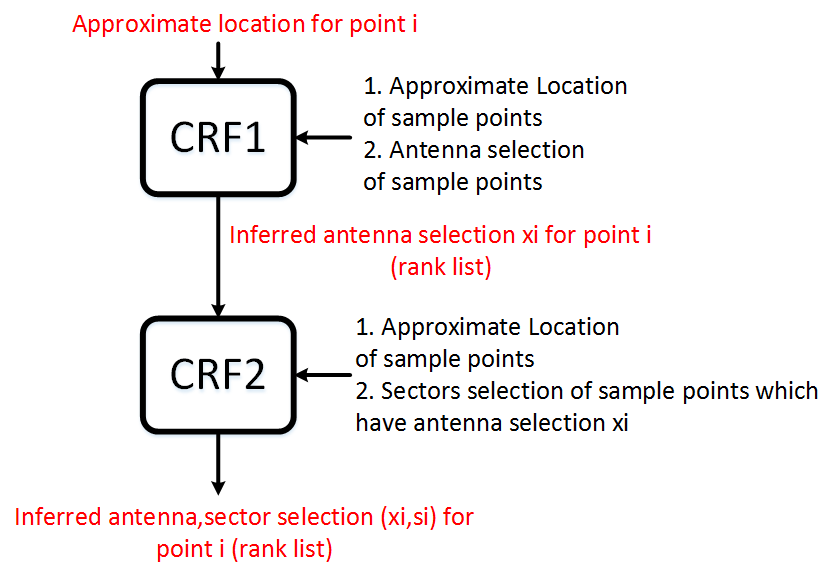
\includegraphics[width=6.5cm,height=4cm]{topology}}
	\caption[U-example]{Topology of Inference Block of AutoBeam}
\end{figure}
\subsection{Inference}
In this section we solve the following question: assume we have the trained CRF1 and CRF2, and the optimal beam selection for some sample points $S$, infer the beam selection for the rest of the points in the grid. More specifically, the beam selection of $v\in V$ contains the following information $(AP\_ID_{v}, Sec\_AP\_ID_{v}, Sec\_UE\_ID_{v})$: the $AP\_ID_{v}$ and $SEC\_AP\_ID_{v}$ is the ID of the AP and transmit sector of AP which generates the maximum SNR at $v$. $SEC\_UE\_ID_{v}$ is the ID of the transmit sector of $UE$ which generates the maximum SNR at AP. We call the two tuple $(Sec\_AP\_ID_{v}, Sec\_UE\_ID_{v})$ \emph{tuple sector} of $v$, and we assign a ID $Sec\_ID_{v}$ to every tuple sector of $v$, the ID can be calculated by using a one-to-one mapping between $Sec\_ID_{v}$ and $(Sec\_AP\_ID_{v}, Sec\_UE\_ID_{v})$. Furthermore, we assume the $SEC\_AP\_ID$ and $SEC\_UE\_ID$ are assigned based on the consecutive physical locations of the sectors. So if the two sectors which are next to each other, their sector IDs are also next to each other. Moreover, the sector with the largest sector ID and smallest sector ID are also next to each other because the sectors are circularly placed. 
 
For the set of samples $S$, we know their optimal beam selections $x^{*}_{S}$. $x^{*}_{s},s\in S$ contains a set of three tuples, $\{(AP\_ID^{*}_{s}, Sec\_AP\_ID^{*}_{s}, Sec\_UE\_ID^{*}_{s})\}$, where $AP\_ID^{*}_{s}, Sec\_AP\_ID^{*}_{s}, Sec\_UE\_ID^{*}_{s}$ is the optimal antenna ID, AP transmit sector ID and UE transmit ID of $v$. For the ease of interpretation, denote $x^{AP\_ID*}_{S}=\{x^{AP\_ID*}_{s\in S}\}=\{(AP\_ID)^{*}_{s\in S}\}$ and $x^{Sec*}_{S}=\{x^{Sec*}_{s\in S}\}=\{(Sec\_AP\_ID^{*}_{s}, Sec\_UE\_ID^{*}_{s}))\}$. 

From subsection C, the output of the CRF inference contains $\{Q(x_{v}|rm)\}$, $\forall v in V, x_{v}\in X$. That is, for every $v\in V$, CRF returns a $|X|\times 1$ probability vector $\vec{Q}_{v}=[Q(x_{v}=1|rm),...,Q(x_{v}=|X||rm)]^\top$ which contains the probability of $x_{v}$ take on every label in $X$. %We call this vector \emph{probability vector} of $v$.    

%Now we will present our solution to the question we proposed above. More specifically, for each point $v\in V$ the Inference block will return a sorted probability vector for beam selection, which lists the beam selections sorted in descending order based on its probability, and we call this sorted probability vector \emph{Beam selection map}. Denote $X^{AP}, X^{Sec}$ the set of all possible AP IDs and tuple sector IDs.
%\begin{algorithm}[H]
%	Input: Beam selections $x_{S}^{*}$ of the sample points, trained CRF1, CRF2 \\
%	Output: Beam selection map $B=\{B_{v},v\in V\}$ and the probability matrix $P=\{P_{v},v\in V\}$ of $v\in V\backslash S$ \\
%	Use $x^{AP*}_{S}$ and CRF1 to calculate the probability vector $\vec{P}^{AP}_{v}$ for AP at each $v\in V$\\
%	\For{each $x\in X^{AP}$}{
%		Denote $S_{x}$ the set of samples which has $AP\_id^{*}=x$, Use $x^{AP*}_{S_{x}}$ and CRF2 to calculate the probability vector for sectors $\vec{P}^{Sec}_{v,AP=x}$ at each $v\in V$.
%	}
%	\For{each $v\in V\backslash S$}{ 
%		\For{each $x\in X^{AP}$}{
%			\For{each $y\in X^{Sec}$}{
%				Calculate $P(x,y) = P(y|x)P(x) = \vec{P}^{Sec}_{v,AP=x}(y)\vec{P}^{AP}_{v}(x)$, where $\vec{P}^{Sec}_{v,AP=x}(y)$ and $\vec{P}^{AP}_{v}(x)$ is the yth and xth element of $\vec{P}^{Sec}_{v,AP=x}(y)$ and $\vec{P}^{AP}_{v}$\\
%				Append $(x,y)$ to $B_{v}$ and $P(x,y)$ to $P_{v}$ \\
%			}		
%       }	
%       Sort $B_{v}$ in descending order\\
%	}
%    Return $B=\{B_{v},v\in V\}$ and $P=\{P_{v},v\in V\}$
%	\caption{Offline Inference Algorithm}
%\end{algorithm}

For each point $v\in V$ the Inference block will return a probability vector for beam selection, which lists each beam selections and its probability, we can define a map with the key equals the beam selection and value equals its probability, we call this map \emph{beam selection map} of $v$, denoted by $B_{v}$, so each entry of $B_{v}$ is a four tuple which comprises  $AP\_ID$,$Sec\_AP\_ID$,$Sec\_UE\_ID$, and its probability. We can also aggregate all the $B_{v}, v\in V$ to get another map $B = \{B_{v},v\in V\}$. Denote $X^{AP}, X^{AP_Sec}$, $X^{UE_Sec}$,$X^{Sec}$ the set of all possible IDs of AP, transmit sectors of AP, transmit sectors of UE and tuple sector IDs, and we assume all the APs have same number of transmit sectors, and so is all the UEs. The offline Inference Algorithm (OIA) is described in Algorithm 2.
\begin{algorithm}[H]
	Input: Set of samples $S$, optimal beam selections $x_{S}^{*}$ of the sample points, trained CRF1, CRF2 \\
	Output: Beam selection maps $B=\{B_{v},v\in V\}$ for $v\in V\backslash S$ \\
	Use $x^{AP*}_{S}$ and CRF1 to calculate the probability vector $\vec{Q}^{AP}_{v}=[Q(AP\_ID_{v}=1|rm),...,Q(AP\_ID_{v}=|X^{AP}||rm)]^\top$ for AP at each $v\in V$\\
	\For{each $x\in X^{AP}$}{
		Denote $S_{x}$ the set of samples which has $AP\_id^{*}=x$, Use $x^{Sec*}_{S_{x}}$ and CRF2 to calculate the probability vector for sectors $\vec{Q}^{Sec}_{v,AP\_ID=x}=[Q(Sec\_ID_{v}=1|AP\_ID=x,rm),...,Q(Sec\_ID_{v}=|X^{Sec}||AP\_ID=x,rm)]^\top$ at each $v\in V$.
	}
	\For{each $v\in V\backslash S$}{ 
		\For{each $x\in X^{AP}$}{
			\For{each $y\in X^{Sec}$}{
				Calculate $P(AP\_ID_{v}=x,Sec\_ID_{v}=y) = P(y|x)P(x) = \vec{P}^{Sec}_{v,AP=x}(y)\vec{P}^{AP}_{v}(x)$, where $\vec{P}^{Sec}_{v,AP=x}(y)$ and $\vec{P}^{AP}_{v}(x)$ is the yth and xth element of $\vec{P}^{Sec}_{v,AP=x}(y)$ and $\vec{P}^{AP}_{v}$\\
				Append $(x,y,P(x,y))$ to $B_{v}$ \\
			}		
		}	
	}
	Return $B=\{B_{v},v\in V\}$
	\caption{Offline Inference Algorithm (OIA)}
\end{algorithm}


\subsection{Training}
For training, we want to find the parameters $\theta = \{w_{k},m_{vv'}\},\forall 1\leq k\leq K, (v,v')\in E$ for CRF1 and CRF2 given the training data. More specifically, denote $D^{AP}_{r}=\{(AP\_id)_{v\in V_{r}}\}$ the set of optimal AP IDs of points in $r$ and $D^{Sec}_{r,AP=x}=\{(Sec\_AP\_id, Sec\_UE\_id)_{v\in V_{r}}\}$,$x\in X^{AP}$ the set of optimal tuple sector IDs of $x$ to make communication, $V_{r}$ denote the set of nodes in $r$. CRF1 and CRF2 can be trained with Offline Training Algorithm (OTA):
\begin{algorithm}[H]
	Input:  $D^{AP}_{r}$ for $1\leq r\leq R$, $D^{Sec}_{r,AP=x}$ for $1\leq r\leq R$ and $x\in X^{AP}$\\
	Output: $\theta = \{w_{k},m_{vv'}\}$ for CRF1 and CRF2\\
    Denote $D^{AP}=\{D^{AP}_{r},1\leq r\leq R\}$. Use $D^{AP}_{r}$ to train CRF1 with Algorithm 1\\
	\For{each $x\in X^{AP}$}{
		Denote $D^{Sec}_{r} = \{D^{Sec}_{r,AP=x},x\in X^{AP}\}$ and $D^{Sec}=\{D^{Sec}_{r},1\leq r\leq R\}$. Use $D^{Sec}$ to train CRF2 with Algorithm 1
	}
    Return $\theta$ for CRF1 and CRF2
	\caption{Offline Training Algorithm (OTA)}
\end{algorithm}
\subsection{Reason for this design}
We use CRF1 to capture the spatial correlation of AP selection across different nodes, and CRF2 to capture the spatial correlation of sector selection across different nodes. There is an alternative design of CRF which integrates CRF1 and CRF2 together and generate a one-shot solution for AP and sector selection. We call this integrated design. However, the integrated design has much more ground truth labels than cascaded design, which equals number of APs$\times$ number of sectors, which dramatically increases the complexity of both inference and training process of CRF.  
\section{Communication Protocol}
In this section, we will discuss the communication protocol used for beamforming. However, since for the SLS phase, we only need to select the coarse-grain transmit sector for AP and UE, which means we only need to select a set of \textbf{consecutive} transmit sectors. We achieve this by defining a \emph{sector range} $\xi\in \mathbbm{Z}^+$, and transfer each unique sector choice to a set of sectors by considering its nearby sectors within $\pm \xi$ range of it. For example, if $y = (Sec\_AP\_id', Sec\_UE\_id')$ is the inferred tuple sector by CRF2, then the corresponding set of sectors are $y_{\xi} = ((Sec\_AP\_id'\ominus \xi_{AP}, Sec\_AP\_id'\oplus \xi_{AP}), (Sec\_UE\_id'\ominus \xi_{AP}, Sec\_UE\_id'\oplus \xi_{AP}))$, where $\xi_{AP},\xi_{Sec}$ are the sector range for AP and UE, and we call $y_{\xi}$ the \emph{enlarged set} of y. Note that modulo addition and subtraction are used because all the sectors are placed in circle, so the sector with maximum and minimum sector ID are next to each other. 
We also define some terms and operations on the beam selection map. Let $f$ denote the entry of $B_{v}$. So $f_{1},f_{2},f_{3},f_{4}$ are the $AP\_ID, Sec\_AP\_ID, Sec\_UE\_ID$ and the probability associated with this entry, define $filter()$ operation to filter $B_{v}$ based on the certain criteria, for example $Filter(AP\_ID=3;B_{v})$ returns all the entries which has AP=3 in $B$. Define  $Sort(B_{v})$ operation to sort $B_{v}$ in the descending order based on the probability of each entry. Define $Sum()$ operation to sum the probabilities of the entries based on the certain criteria. For example, $Sum(AP;B_{v})$ will return a summation based on each $AP\_ID$ of $B_{v}$, the ith entry of $Sum(AP)$ will contain the summation of the probabilities of all the entries whose $AP\_ID=i$. Finally, define $Remove()$ operation to remove the entry. For example $Remove((2, 3, 4);B_{v})$ will remove the entry with $AP\_ID=1,Sec\_AP\_ID = 2, Sec\_UE\_ID=3$ from $B_{v}$.
\subsection{Sort the beam selection map}
First we have to find the optimal AP ID together with its transmit sector ID to make communication from AP to UE (Figure 3). To achieve this, we will sort the beam selection map based on the $AP\_id$ and $Sec\_AP\_id$ features. Assume we do beamforming at node $v$, and denote $X^{Sec_{AP}}, X^{Sec_{UE}}$ the set of transmit sector IDs of AP and UE, the offline sorting algorithms (OSA) is described in Algorithm 3.
\begin{algorithm}[H]
	Input: beam selection map $B_{v}$ of $v$\\ 
	Output: $B^{AP\_Sec}_{v}$
	\For{each $x\in X^{AP}$}{
		\For{each $y\in X^{AP_Sec}$}{
			Calculate $P(AP\_ID =x,Sec\_AP\_ID = y)=P(Filter(AP\_ID = x, Sec\_AP\_ID = y;B_{v})) = \sum\limits_{f\in Filter(AP\_ID = x, Sec\_AP\_ID = y)}f_{4}$\\
			Append $(x,y,P(x,y))$ to $B^{AP\_Sec}_{v}$ \\
			$Sort(B^{AP\_Sec}_{v})$
		}		
	}	
	Return $B^{AP\_Sec}_{v}$
	\caption{Offline Sorting Algorithm (OSA)}
\end{algorithm}
\subsection{Communication Protocol of Beamforming}
After getting $B^{AP\_Sec}_{v}$, we are ready for presenting the protocol of beamforming for a single point, which is described as follows:(Again, we assume that AP and UE already know $B^{AP\_Sec}_{v}$ and $B_{v}$ through WiFi communication) 
\begin{algorithm}[H]	
    Input: $B^{AP\_Sec}_{v}$ and $B_{v}$, sector ranges $\xi_{AP},\xi_{Sec}$ for AP and UE\\
    Set $Update\_with\_erasure = 0$\\
	\For{each $f \in B^{AP\_Sec}_{v}$}{
		\eIf{$f_{4}>P_{TH}$}{
		    $ACK = AP\_sector\_train(f_{1},f_{2},\xi_{AP})$\\
		    \If{$ACK = 1$}{
		    	$B^{UE\_Sec}_{v} = Sum(Sec\_UE\_ID;B^{AP\_Sec}_{v})$
		    	$Sort(B^{UE\_Sec}_{v})$\\   % AP will transmit this to UE 
	            \For{each $f \in B^{UE\_Sec}_{v}$}{
	                \eIf{$f_{2}>P_{TH}$}{
	                    $ACK = UE\_sector\_train(f_{1},f_{2},\xi_{Sec})$\\
	                    \If{$ACK = 1$}{Break}
	                }
	                {
	                	Find the UE transmit sector with the scheme of 802.11ad\\
	                	Set $Update\_with\_erasure$ = 1 \\
	                	Break
	                }
	            }
		    }
		}
		{
		    Find the AP and UE transmit sector with the scheme of 802.11ad\\
		    Set $Update\_without\_erasure = 1$ \\
		    Break
		}  
	}
    Proceed to beam refinement phase, find the optimal AP ID and sector ID $(AP\_ID^{*}_{v}, Sec\_AP\_ID^{*}_{v}, Sec\_UE\_ID^{*}_{v})$\\
    Append $v$ to $S$, and $(AP\_ID^{*}_{v}, Sec\_AP\_ID^{*}_{v}, Sec\_UE\_ID^{*}_{v})$ to $x_{S}^{*}$\\
    \If{$Update\_with\_erasure = 1$}{Clear the samples whose location is within $\beta$ meters of $v$}
    $B=OIA(S,x_{S}^{*},CRF1,CRF2)$\\
    \For{each $v\in V$} {$B^{AP\_Sec}_{v}= OSA(B_{v})$}
	\caption{Communication Protocol of Beamforming (CPB)}
\end{algorithm}

During $AP\_sector\_train(f_{1},f_{2},\xi_{AP})$, the corresponding antenna $f_{1}$ will transmit frames through sectors $[f_{2}\ominus \xi_{AP},f_{2}\oplus \xi_{AP}]$, each frame is labeled with the corresponding sector ID. If UE does not receive the frames from AP, it broadcast with a ACK frame with ACK = 0 through WiFi after RTT, so that all the APs can receive this ACK. The ACK frame also contains the index of the next entry in $B_{v}^{AP\_Sec}$. Once AP receive this ACK frame, the next pair of $f_{1},f_{2}$ will be tried based on Algorithm 5 (Figure $9(a)$). If UE receives the frames with satisfied SNR, it reply with a ACK frame with ACK = 1 through WiFi (Figure $9(b)$). After AP receiving the ACK frame, it will send the $B^{UE\_Sec}_{v}$, which contains a ranked list of UE transmit sectors to UE through mm-wave band (Figure $9(c)$). 
\begin{figure}
	\centerline{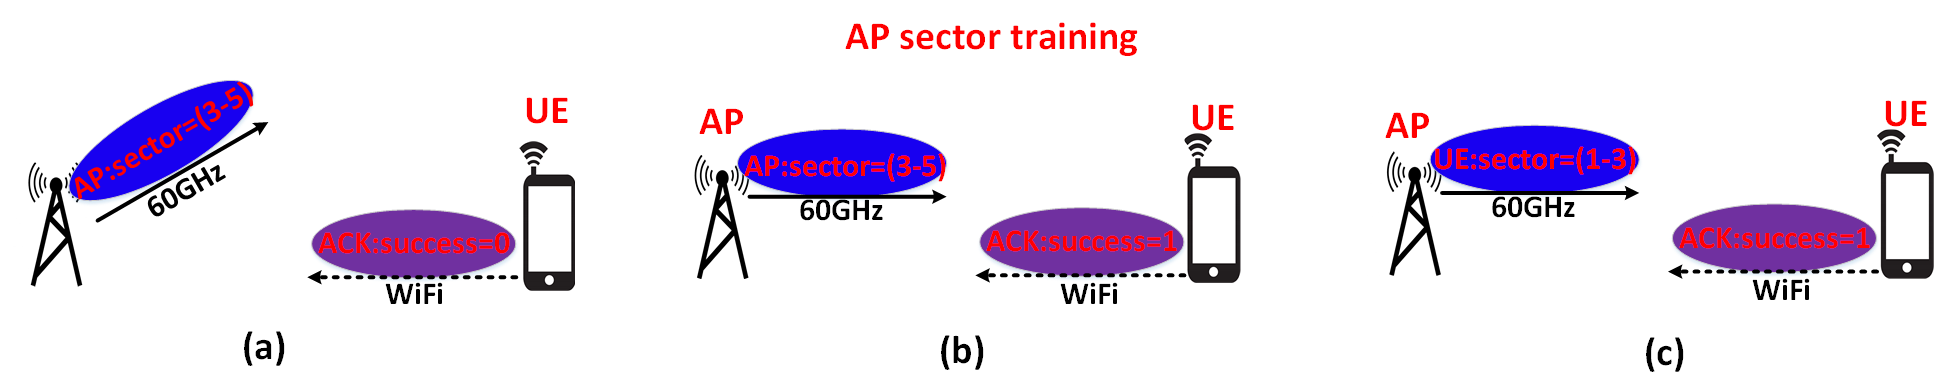
\includegraphics[width=8.5cm,height=2cm]{ap_sector_training}}
	\caption[U-example]{AP transmit sector training procedure}
\end{figure}
Similarly, for $UE\_sector\_train(f_{1},f_{2},\xi_{Sec})$, the UE will transmit frames through sectors $[f_{2}\ominus \xi_{Sec},f_{2}\oplus \xi_{Sec}]$, each frame is labeled with the corresponding sector ID. If AP receives the frames with enough SNR, it reply with a ACK frame with success = 1 through mm-wave band (Figure $10(a)$), since the connection from AP to UE is already set up (? Receiver sector training). If AP does not receive the frames from AP, it reply with a ACK frame with success = 0 through mm-wave band after RTT (Figure $10(b)$). Once AP receive this ACK frame, the next $f_{1}$ will be tried as indicated in Algorithm 1. 
 \begin{figure}
 	\centerline{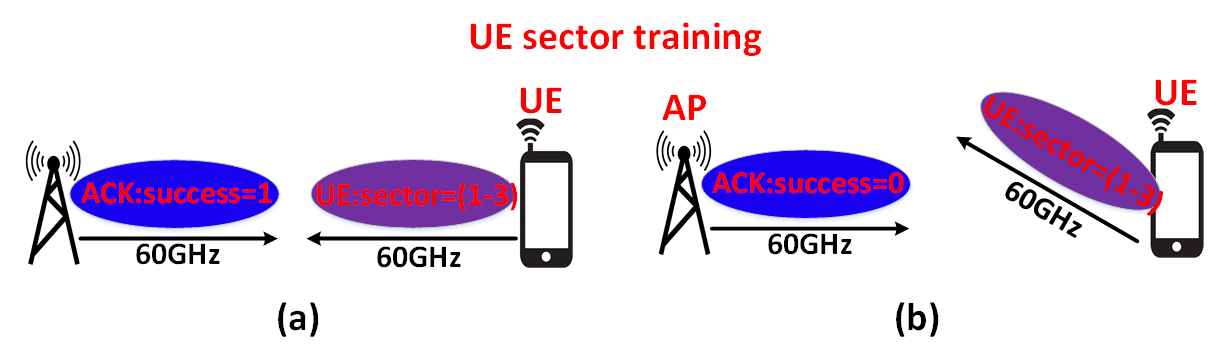
\includegraphics[width=6.5cm,height=2cm]{ue_sector_training}}
 	\caption[U-example]{UE transmit sector training procedure}
 \end{figure}
Start from beginning, AP will calculate the joint probability for each $(AP\_ID,Sec\_AP\_ID)$, and rank them in descending order based on the probabilities, AP will try each $(AP\_ID,Sec\_AP\_ID)$ with $AP\_sector\_train$. If several pairs have been tried and the probability of $(AP\_ID,Sec\_AP\_ID)$ is lower than $P_{TH}$, traditional 802.11ad scheme will be used for SLS. If $(AP\_ID^{*},Sec\_AP\_ID^{*})$ is found to be good and its probability is greater than $P^{1}_{TH}$. All the entries which has $AP\_ID=AP\_ID*$ and $Sec\_AP\_ID=Sec\_AP\_ID^{*}$ will be filtered and the joint probability $P(AP\_ID^{*},Sec\_AP\_ID^{*},Sec\_UE\_ID)$ will be calculated for each $Sec\_UE\_ID$. Since $P(AP\_ID^{*},Sec\_AP\_ID^{*})$ is a constant, we have $P(AP\_ID^{*},Sec\_AP\_ID^{*},Sec\_UE\_ID)\propto P(Sec\_UE\_ID|AP\_ID^{*},Sec\_AP\_ID^{*})$. Then the entries will be ranked in descending order based on the joint probability and UE will try each $Sec\_UE\_ID$ with $UE\_sector\_train$.  If several pairs have been tried and the probability of $P(AP\_ID*,Sec\_AP\_ID*,Sec\_UE\_ID)$ is lower than $P^{2}_{TH}$, traditional 802.11ad scheme will be used for SLS from UE to AP.  
\subsection{Online Communication Protocol for Beam Adjustment}
AutoBeam also enables fast beam adjustment when environment changes (i.e. human blockage), the protocol is described in Algorithm 6.
\begin{algorithm}[H]	
	\While{1}{
		Measure the throughput $\alpha_{v}$ for UE located at $v$ over time period $t$
        \If{$\alpha_{t}<\alpha_{TH}$}{
        	$Remove((AP\_ID^{*}_{v}, Sec\_AP\_ID^{*}_{v}, Sec\_UE\_ID^{*}_{v});B_{v})$, normalize the probabilities in $B_{v}$ to make their sum equals 1;\\
            $B^{AP\_Sec}_{v}= OSA(B_{v})$\\
            $CPB(B^{AP\_Sec}_{v},B_{v}$)
        }
	}
	\caption{Online Communication Protocol for Beamforming (OCPB)}
\end{algorithm}
In $OCPB$, if the throughput (both sides?) $\alpha_{v}$  of $v$ is less than a threshold $\alpha_{TH}$, the beam adjustment process will be triggered. It removes the current beam selection from the beam selection map $B_{v}$, and perform OSA and CPB. The state diagrams for online and offline operation is shown Figure 11 and Figure 12.

\begin{thebibliography}{1}

\bibitem{IEEEhowto:kopka}
N. Gude, T. Koponen, J. Pettit, B. Pfaff, M. Casado, N. McKeown, and
S. Shenker. \emph{"NOX: towards an operating system for networks"}, ACM
SIGCOMM Computer Communication Review, 38(3):105–110, July 2008.

\bibitem{IEEEhowto:kopka}
H. H. Liu, X. Wu, M. Zhang, L. Yuan, R. Wattenhofer, and D.A.Maltz. \emph{"zUpdate: Updating data center networks with zero loss"}, in Proceedings of ACM Sigcomm, 2013.
\bibitem{IEEEhowto:kopka}
S.~Floyd, M.~Handley, J.~Padhye, J.~Widmer. \emph{"Equation-Based Congestion Control for Unicast Applications"}, in Proceedings of ACM Sigcomm, 2000.
\bibitem{IEEEhowto:kopka}
L.~Vicisano, J.~Crowcroft, L.~Rizzo. \emph{"TCP-like congestion control for layered multicast data transfer"}, in Proceedings of Infocom, 1998.
\bibitem{IEEEhowto:kopka}
J.~Dean, S.~Ghemawat. \emph{"MapReduce: simplified data processing on large clusters"}, in Proceedings of OSDI, 2004.
\bibitem{IEEEhowto:kopka}
A.~Shribman, B.~Hudzia. \emph{"Pre-Copy and post-copy VM live migration for memory intensive applications"}, in Proceedings of Euro-Par, 2012.
\bibitem{IEEEhowto:kopka}
X.~Chen, HM.~Jones, ADS.~Jayalath. \emph{"Congestion-aware routing protocol for mobile ad hoc networks"}, in Proceedings of VTC, 2007.
\bibitem{IEEEhowto:kopka}
JW.~Jiang, T.~Lan, S.~Ha, M.~Chen, \emph{"Joint VM placement and routing for data center traffic engineering"}, in Proceedings of Infocom, 2012.
\bibitem{IEEEhowto:kopka}
A. R. Curtis, J. C. Mogul, J. Tourrilhes, P. Yalagandula, P. Sharma and S. Banerjee. \emph{"DevoFlow: Scaling flow management for high-performance networks”}, in Proceedings of in ACM Sigcomm, 2011.
\bibitem{IEEEhowto:kopka}
M. Yu, J. Rexford, M. J. Freedman, and J. Wang. \emph{"Scalable Flow-Based Networking with DIFANE"}. In Proceedings of Sigcomm, 2010.
\bibitem{IEEEhowto:kopka}
R.~Wang,D.~Butnariu,J.~Rexford. \emph{"OpenFlow-based server load balancing gone wild"}. In proceedings of USENIX Hot-Ice, 2011
\bibitem{IEEEhowto:kopka}
M. Alizadeh, A. Greenberg, D. A. Maltz, J. Padhye, P. Patel, B. Prabhakar, S. Sengupta and M. Sridharan. \emph{"Data Center TCP (DCTCP)"}, in Proceedings of ACM Sigcomm, 2010.
\bibitem{IEEEhowto:kopka}
X.~Liu, R.~Meiners,E.~Torng. \emph{"TCAM Razor: A Systematic Approach Towards Minimizing Packet Classifiers in TCAMs"}. IEEE/ACM transaction on networking, VOL. 18, NO. 2, APRIL 2010.
\bibitem{IEEEhowto:kopka}
S.Yeganeh, Y.Ganjali. \emph{"Kandoo: a framework for efficient and scalable offloading of control applications"}, in Proceedings of ACM HotSDN, 2012.
\bibitem{IEEEhowto:kopka}
A.S Tam, X.Kang and H.J.Chao. \emph{"Use of devolved controllers in data center networks"}, in Proceedings of Infocom Computer Communications Workshops, 2011.
\bibitem{IEEEhowto:kopka}
K. Phemius, M. Bouet and J. Leguay. \emph{"DISCO: Distributed multi-domain SDN controllers"}, in Proceedings of IEEE NOMS, 2014.
\bibitem{IEEEhowto:kopka}
Y. Jimenez, C. Cervello-Pastor and A.J.Garcia. \emph{"On the controller placement for designing a distributed SDN control layer"}, in Proceedings of IFIP Networkings, 2014.
\bibitem{IEEEhowto:kopka}
M.~Reitblatt,N.~Foster,J.~Rexford,D.~Walker. \emph{"Consistent updates for software-defined networks: change you can believe in!"}, in Proceedings of the 10th ACM Workshop on Hot Topics in Networks, 2011.
\bibitem{IEEEhowto:kopka}
M.~Reitblatt, N.~Foster, J.~Rexford, C.~Schlesinger. \emph{"Abstractions for network update"},  in Proceeding Sigcomm, 2012.
\bibitem{IEEEhowto:kopka}
C.Y. Hong, S.Kandula, R.Mahajan, M.Zhang, V.Gill, M.Nanduri, R.Wattenhofer. \emph{"Achieving high utilization with software-driven WAN"}, in Proceedings of Sigcomm, 2013.
\bibitem{IEEEhowto:kopka}
X.~Jin, HH.~Liu, R.~Gandhi, S.~Kandula. \emph{"Dynamic scheduling of network updates"},
in Proceeding Sigcomm, 2014. 
\bibitem{IEEEhowto:kopka}
W. Cui, I. Stoica, R.H. Katz. \emph{"Backup path allocation based on a correlated link failure probability model in overlay networks"}, in Proceedings of ICNP, 2002.
\bibitem{IEEEhowto:kopka}
V.Y. Liu, D. Tipper. \emph{"Spare capacity allocation using shared backup path protection for dual link failures"}, in Proceedings of Design of Reliable Communication Networks (DRCN), 2011.
\bibitem{IEEEhowto:kopka}
B. Jozsa, O. Daniel, A. Kern. \emph{"Surviving multiple network failures using shared backup path protection"}, in Proceedings of ISCC, 2003.
\bibitem{IEEEhowto:kopka}
S. Lee, K.Y. Li, K.Y. Chan, G.H. Lai, and Y.C. Chung. \emph{"Path
layout planning and software based fast failure detection in survivable OpenFlow networks"}, in Proceedings of Design of Reliable Communication Networks (DRCN), 2014.
\bibitem{IEEEhowto:kopka}
S. Sharma, D. Staessens, D. Colle, M. Pickavet, and P. Demeester. \emph{"Enabling Fast Failure
Recovery in OpenFlow Networks"}, in Proceedings of DRCN, 2011.
\bibitem{IEEEhowto:kopka}
V. Adrichem, V. Asten and  F.A. Kuipers. \emph{"Fast Recovery in Software-Defined Networks"}, in Proceedings of Software Defined Networks (EWSDN), 2014.
\bibitem{IEEEhowto:kopka}
M. Reitblatt, M. Canini, A. Guha, and N. Foster. \emph{"FatTire: Declarative Fault Tolerance
for Software-Defined Networks"}, in Proceedings of ACM HotSDN, 2013.
\bibitem{IEEEhowto:kopka}
"Openflow specification" : https://www.opennetworking.org/images/stories/\\downloads/sdn-resources/onf-specifications/openflow/openflow-spec-v1.3.0.pdf
\bibitem{IEEEhowto:kopka}
H. Jiang and C. Dovrolis, \emph{"Why is the internet traffic bursty in short time scales?"}, in Proceedings of ACM Sigmetrics, 2005.
\bibitem{IEEEhowto:kopka}
T. Benson, A. Anand,  A. Akella and M. Zhang. \emph{"Understanding data center traffic characteristics"}, ACM SIGCOMM Computer Communication Review archive Volume 40 Issue 1, January 2010.
\bibitem{IEEEhowto:kopka}
DP.~Williamson, DB. Shmoys. "The Design of Approximation Algorithms": http://www.designofapproxalgs.com/ 
\bibitem{IEEEhowto:kopka}
\emph{"Modeling Topology of Large Internetworks"}: http://www.cc.gatech.edu/projects/gtitm/
\bibitem{IEEEhowto:kopka}
N. Spring, R. Mahajan, D. Wetherall, and T. Anderson, \emph{"Measuring ISP
Topologies with Rocketfuel}, IEEE/ACM Transactions on Networking, vol. 12, no. 1, pp. 2–16, February 2004.
\bibitem{IEEEhowto:kopka}
A. Nucci, A. Sridharan and N. Taft. \emph{"The problem of synthetically generating IP traffic matrices: initial recommendations"}, ACM SIGCOMM Computer Communication Review Homepage archive
Volume 35 Issue 3, July 2005, Pages 19-32. 
\bibitem{IEEEhowto:kopka}
T. Hirayama, S. Arakawa, S. Hosoki, and M. Murata, \emph{"Models of link
capacity distribution in ISP’s router-level topologies"}, JCNC, vol. 3, pp. 205–216, 2011.
 
\end{thebibliography}
\end{document}

